\documentclass[11pt,twoside]{article}
\usepackage[utf8]{inputenc}
\usepackage[T1]{fontenc}

% Page margins, header and footer positions
\usepackage{geometry}
\geometry{
 a4paper,
 total={210mm,297mm},
 left=25mm,
 right=25mm,
 top=30mm,
 bottom=25mm,
 headsep=7mm
}

\interfootnotelinepenalty=10000

% To display filling dots in the TOC for all entries
\usepackage[titles]{tocloft}
\renewcommand{\cftsecleader}{\cftdotfill{\cftdotsep}}

% Define new header and footer style
\usepackage{fancyhdr}

\pagestyle{fancy}
\fancyhf{}
\lhead{\color{Gray}{\small{Bogdanovic Stefan, Rodari Simone, Pignataro Gabriele}}}
\lfoot{\textcolor{Gray}{\small{Copyright © 2024, Bogdanovic Stefan, Rodari Simone, Pignataro Gabriele – All rights reserved}}}
\rfoot{\textcolor{Gray}{\thepage}}
\renewcommand{\headrulewidth}{0pt}

% PACKAGES
\usepackage{wasysym}
\usepackage{pifont}
\usepackage{minted}

\newcommand{\supported}{\ding{52}\xspace}
\newcommand{\unsupported}{\ding{55}\xspace}
\newcommand{\partsupported}{\textcolor{black!40}{\ding{52}}\xspace}
\newcommand{\lowsupported}{\textcolor{black!20}{\ding{52}}\xspace}
\newcommand{\unknowsupported}{\textbf{?}\xspace}

% Font: Times
\usepackage{times}
% Change monospaced font
\renewcommand{\ttdefault}{lmtt}

% Tables
\usepackage{tabu}
\usepackage{tabularx}
\usepackage{ltablex}
\usepackage{longtable}
\usepackage{float}

% Landscape mode
\usepackage{pdflscape}
\usepackage{rotating}
\usepackage{caption}

% Make landscape mode be sensitive to even and odd pages
\def\myrotate{\ifodd\c@page\else-\fi 90}
\makeatletter
\global\let\orig@begin@landscape=\landscape%
\global\let\orig@end@landscape=\endlandscape%
\gdef\@true{1}
\gdef\@false{0}
\gdef\landscape{%
    \global\let\within@landscape=\@true%
    \orig@begin@landscape%
}%
\gdef\endlandscape{%
    \orig@end@landscape%
    \global\let\within@landscape=\@false%
}%
\@ifpackageloaded{pdflscape}{%
    \gdef\pdf@landscape@rotate{\PLS@Rotate}%
}{
    \gdef\pdf@landscape@rotate#1{}%
}
\let\latex@outputpage\@outputpage
\def\@outputpage{
    \ifx\within@landscape\@true%
        \if@twoside%
            \ifodd\c@page%
                \gdef\LS@rot{\setbox\@outputbox\vbox{%
                    \pdf@landscape@rotate{-90}%
                    \hbox{\rotatebox{90}{\hbox{\rotatebox{180}{\box\@outputbox}}}}}%
                }%
            \else%
                \gdef\LS@rot{\setbox\@outputbox\vbox{%
                    \pdf@landscape@rotate{+90}%
                    \hbox{\rotatebox{90}{\hbox{\rotatebox{0}{\box\@outputbox}}}}}%
                }%
            \fi%
        \else%
            \gdef\LS@rot{\setbox\@outputbox\vbox{%
                \pdf@landscape@rotate{+90}%
                \hbox{\rotatebox{90}{\hbox{\rotatebox{0}{\box\@outputbox}}}}}%
            }%
        \fi%
    \fi%
    \latex@outputpage%
}
\makeatother

% Graphics
\usepackage{graphicx}
\usepackage[dvipsnames, table]{xcolor}

% Other
\usepackage{ifthen}
\usepackage{xspace}
\usepackage{enumitem}
\usepackage{amssymb}
\usepackage[pdftex, colorlinks]{hyperref}
\newcommand{\comment}[1]{{\color{Black}$\blacktriangleright$ Comment: #1 $\blacktriangleleft$}}

% Some utilities
\input{util/highlight}
\input{util/abbrev}

% TABLE UTILS
\newcommand{\uctab}[6]{
\begin{tabular}{|m{3cm}|p{9cm}|}
    \hline
    Name & #1 \\
    \hline
    Actors & #2 \\
    \hline
    Entry condition & #3 \\
    \hline
    Event flow & #4 \\
    \hline
    Exit condition & #5 \\
    \hline
    Exception & #6 \\
    \hline
\end{tabular}
}

\newcommand{\rmtab}[2]{
\begin{center}
\begin{tabular}{|p{0.4\textwidth}|p{0.4\textwidth}|}
    \hline
    Requirements & #1 \\
    \hline
    Components & #2 \\
    \hline
\end{tabular}
\end{center}
}

\newcommand{\reqmap}[1]{
\begin{tabular}{|p{0.5\textwidth}|p{0.5\textwidth}|}
    \hline
    #1
    \hline
\end{tabular}
}

%%%%%%%%%%%%%%%%%%%%%%%%%%%%%%%%%%%%%%%%%%%%%%%%%

\begin{document}

% TITLE PAGE
\begin{titlepage}
% LOGO
{\begin{table}[t!]
\centering
\begin{tabu} to \textwidth { X[1.3,r,p] X[1.7,l,p] }
\textcolor{Blue}
{\textbf{\small{Bogdanovic Stefan, Rodari Simone, Pignataro Gabriele}}} & 
\includegraphics[scale=0.5]{Images/PolimiLogo}
\end{tabu}
\end{table}}~\\ [7cm]

% TITLE 
\begin{flushleft}
{\textcolor{Blue}{\textbf{
    \Huge{Students\&Companies} \\
    \LARGE{Design Document}}}} \\ [1cm]
\end{flushleft}
\end{titlepage}

% Define deliverable specific info
\begin{table}[h!]
\begin{tabu} to \textwidth { X[0.3,r,p] X[0.7,l,p] }
\hline
\textbf{Deliverable:} & DD\\
\textbf{Title:} & Students\&Companies \\
\textbf{Authors:} & Bogdanovic Stefan, Rodari Simone, Pignataro Gabriele \\
\textbf{Version:} & 1.0 \\ 
\textbf{Date:} & 07-January-2025 \\
\textbf{Download page:} & \href{https://github.com/SimoPolimi/RodariPignataroBogdanovic}{https://github.com/SimoPolimi/RodariPignataroBogdanovic} \\
\textbf{Copyright:} & Copyright © 2025, Bogdanovic Stefan, Rodari Simone, Pignataro Gabriele – All rights reserved \\
\hline
\end{tabu}
\end{table}

\setcounter{page}{2}

\newpage
\addcontentsline{toc}{section}{Table of Contents}
\tableofcontents
\newpage
\addcontentsline{toc}{section}{List of Figures}
\listoffigures
\addcontentsline{toc}{section}{List of Tables}
\listoftables

\clearpage
{\color{Blue}{\section{Introduction}}}
\label{sect:introduction}
\subsection{Purpose}
Internships are a vital bridge between academic learning and professional experience, providing students with opportunities to apply their skills and companies with access to emerging talent. However, finding the right match between students and internships can be a complex and inefficient process. The Students\&Companies (S\&C) platform addresses these challenges by providing an integrated system that connects university students with companies offering internships. S\&C provides a wide range of features offering a seamless experience for students from the search of an internship to its completion and for companies an easy way to advertise their internship projects. The platform also lets universities to monitor and support their students throughout their internship, overseeing its execution and supporting the involved parties, should problems arise.
\subsection{Scope}
The Students\&Companies platform provides its services to different users, identifiable into three main classes: students,  companies and universities. Each one of them has different roles and interacts with the system in various ways.
S\&C is aimed mainly at university students that want to take part in an internship program, as they can search for new internships suiting their preferences or let the system inform them when internships matching their profile are available. S\&C is also able to provide suggestions on how to improve their profile to make it more appealing to companies.
The platform also supports companies easing the internships’ management. In doing so S\&C can be used to create questionnaires to select the most suitable candidates for an internship. Similarly to the suggestions for students, the system can analyze the internship offer to identify eventual improvements that can be made.
Hopefully, every internship comes to an end without problems but if that is not the case, interns and companies can communicate through the platform possibly involving the intern’s alma mater as a supervisor which can also terminate the internship if the parties cannot resolve the controversy.

\subsection{Definitions, Acronyms, Abbreviations}
\subsubsection{Definitions}
\begin{itemize}
    \item \textbf{Recommendations}: Process in which the system informs students when an internship that might interest them becomes available and can inform companies about the availability of student CVs corresponding to their needs.
    \item \textbf{SheerID}\cite{sheerid}: Platform that offers an API to verify students by using their academic credentials.
    \item \textbf{Contract}: The contract represents the lifecycle of an internship application, from initiation to its conclusion.
\end{itemize}
\subsubsection{Acronyms}
\begin{itemize}
    \item \textbf{S\&C}: Students \& Companies
    \item \textbf{DAO}: Data Accessing Object
    \item \textbf{API}: Application Programming Interface
    \item \textbf{REST}: REpresentational State Transfer
\end{itemize}
\subsubsection{Abbreviations}
\begin{itemize}
    \item \textbf{R*}: functional requirements.
\end{itemize}
\subsection{Revision History}
\begin{itemize}
    \item 07/01/2025 - Version 1.0.
\end{itemize}
\subsection{Reference Documents}
\begin{itemize}
    \item Assignment document “Assignment RDD AY 2024-2025.
\end{itemize}
\subsection{Document Structure}
\textbf{Introduction}: Provides a brief description of the project, focusing on the reasons behind its development and the goals to be achieved, as previously explained in the RASD.
Architectural Design: This section describes the architecture at different levels of granularity. \\
\textbf{User Interface Design}: This part presents the wireframes that represent the platform’s user interface. \\
\textbf{Requirements Traceability}: Explains how the goals defined in the previous document are fulfilled through the interaction between the requirements and the components described in this document. \\
\textbf{Implementation, Integration, and Test Plan}: Provides details about the implementation, integration, and testing processes, useful for developers and platform producers. \\
\textbf{Effort Spent}: Shows the effort involved in writing this document. \\
\textbf{Bibliography}: Contains references to any documents and software used to write this paper.

\clearpage
{\color{Blue}{\section{Architectural Design}}}
\label{sect:architectural}
\subsection{Overview}
This section is intended to explain in detail all the components used by the system in order to offer all the functionalities.\\
The figure \ref{fig:hilvl} below shows the high-level architecture of the system-to-be. All the components are better explained in the following paragraphs.\\
\begin{figure}[h]
    \centering
    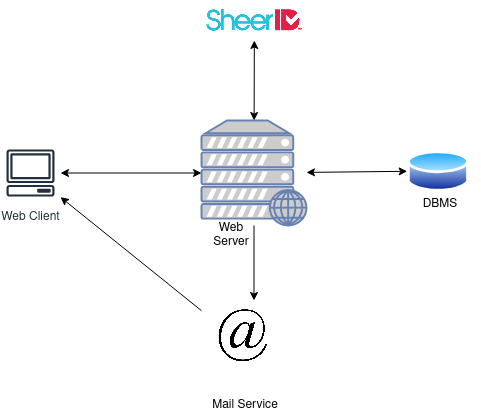
\includegraphics[width=1\linewidth]{Images/S&C_DD-High Level System Overview.drawio.png}
    \caption{High level architecture}
    \label{fig:hilvl}
\end{figure}

\subsection{Component view}
The Students\&Companies platform will be implemented using a three tier architecture. Figure \ref{fig:compview} shows the component view diagram of the platform. The WebApp (presentation layer) will use functions implemented in the business layer through API calls. The business layer interacts with SheerID for the student login functionality.\\
\begin{figure}[h]
    \centering
    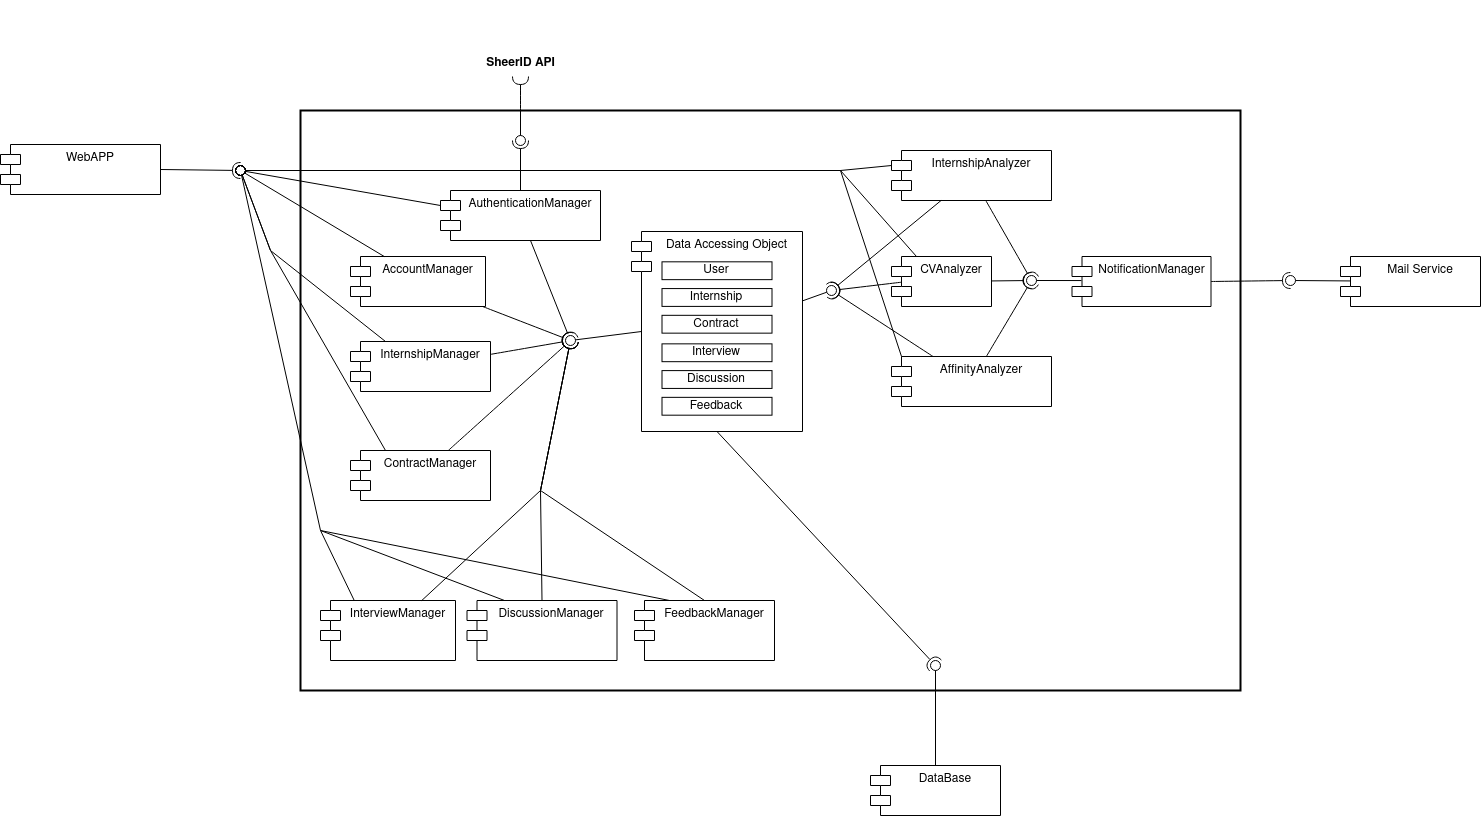
\includegraphics[width=1\linewidth]{Images/comp_view.png}
    \caption{Component view of the system}
    \label{fig:compview}
\end{figure}\\
The system is comprised of the following components:
\begin{itemize}
    \item \textbf{Data Accessing Object (DAO)}: a set of classes utilized to interact with the database, facilitating the retrieval and uploading of information. This approach ensures a single component manages the database connection and handles the query language.
    \item \textbf{AuthenticationManager}: component used for managing user’s registration and login. It uses DAO’s interfaces to manage companies and universities information and SheerID’s API to manage students’ login.
    \item \textbf{AccountManager}: component used to allow the user to modify his profile.
    \item \textbf{InternshipManager}: component used to help users to manage internships.
    \item \textbf{ContractManager}: component used to help users to manage contract stipulations.
    \item \textbf{InterviewManager}: component used to help users to manage interviews.
    \item \textbf{DiscussionManager}: component used to help users to manage discussions.
    \item \textbf{FeedbackManager}: component used to help users to manage feedback.
    \item \textbf{InternshipAnalyzer}: component that produces analytics on internship descriptions based on info collected from the database through DAOs. It relies on the NotificationManager to send notifications to final users.
    \item \textbf{CVAnalyzer}: component that produces analytics on CVs based on info collected from the database through DAOs. It relies on the NotificationManager to send notifications to final users.
    \item \textbf{AffinityAnalyzer}: component that produces analytics on CVs and internship positions based on info collected from the database through DAOs. It relies on the NotificationManager to send notifications to final users.
    \item \textbf{NotificationManager}: component used to abstract the service used to send notifications from the other components.
\end{itemize}

\subsection{Deployment view}
The organization of S\&C's physical infrastructure is shown in figure \ref{fig:deployment}. As it is possible to see, the system uses a single server to host the database, while an array of replicated servers runs the components related to the buisness logic.\\
\begin{figure}[h]
    \centering
    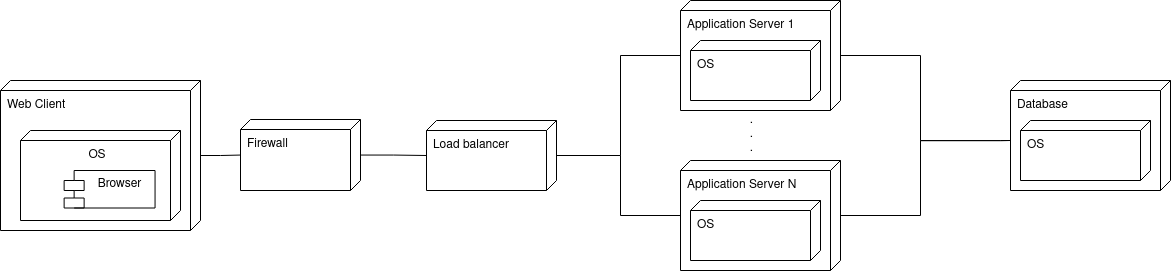
\includegraphics[width=1\linewidth]{Images/deployment.png}
    \caption{Deployment view}
    \label{fig:deployment}
\end{figure}\\
In more detail, the system architecture is made of:
\begin{itemize}
    \item \textbf{WebClient}: the user's device, running a browser which is used to interact with the system.
    \item  \textbf{Firewall}: a firewall to protect the system from potential malicious attacks.
    \item \textbf{Load balancer}: a component used to distribute incoming requests to different replicated servers based on individual loads.
    \item \textbf{Application server}: the server in charge of handling requests from the clients. To ensure acceptable performance even under high loads this server is replicated.
    \item \textbf{Database}: a server dedicated to run the DBMS.
\end{itemize}





\subsection{Runtime View}
[UC1] - Company Registration\newline
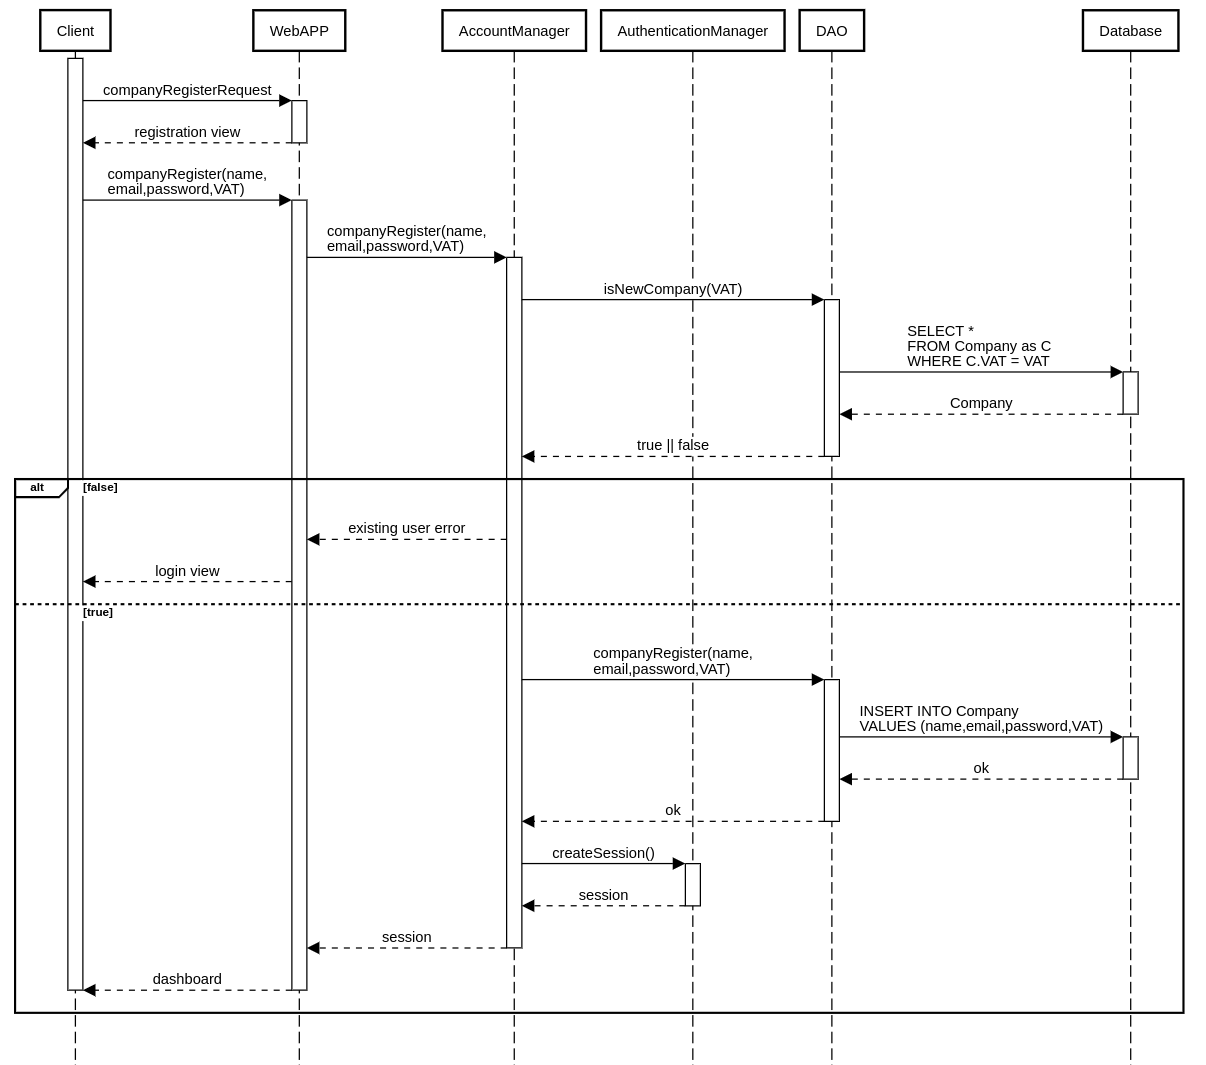
\includegraphics[width=\textwidth]{Images/UC diagrams/company_registration.png}\newpage
[UC2] - Company Login\newline
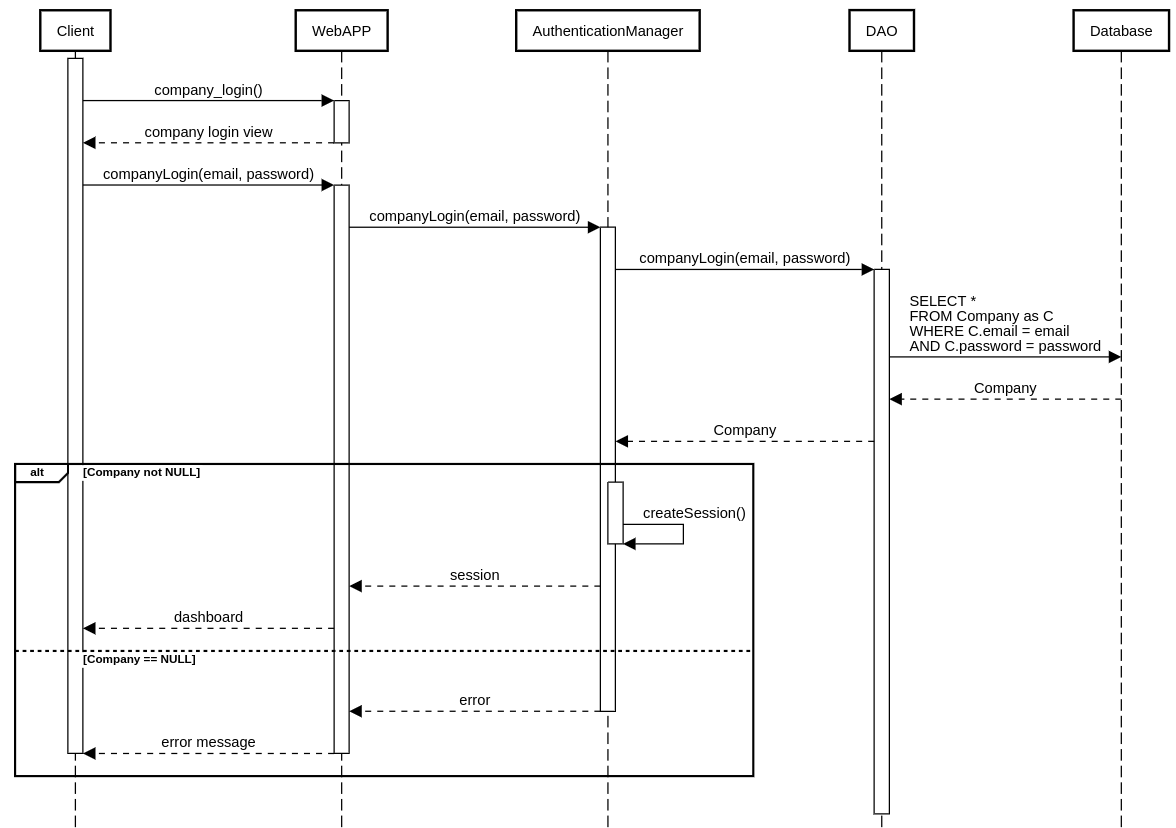
\includegraphics[width=\textwidth]{Images/UC diagrams/company_login.png}\newline
[UC3] - University Login\newline
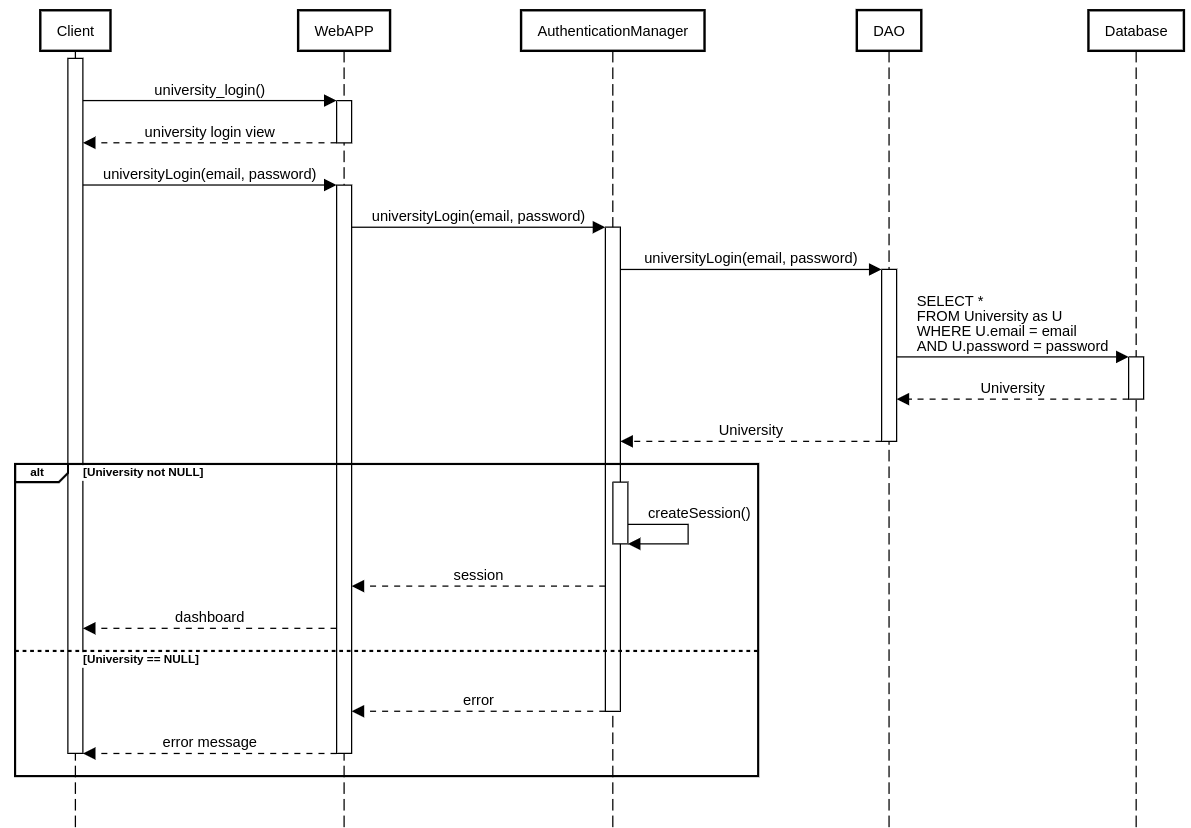
\includegraphics[width=\textwidth]{Images/UC diagrams/university_login.png}\newpage
[UC4] - Student Login\newline
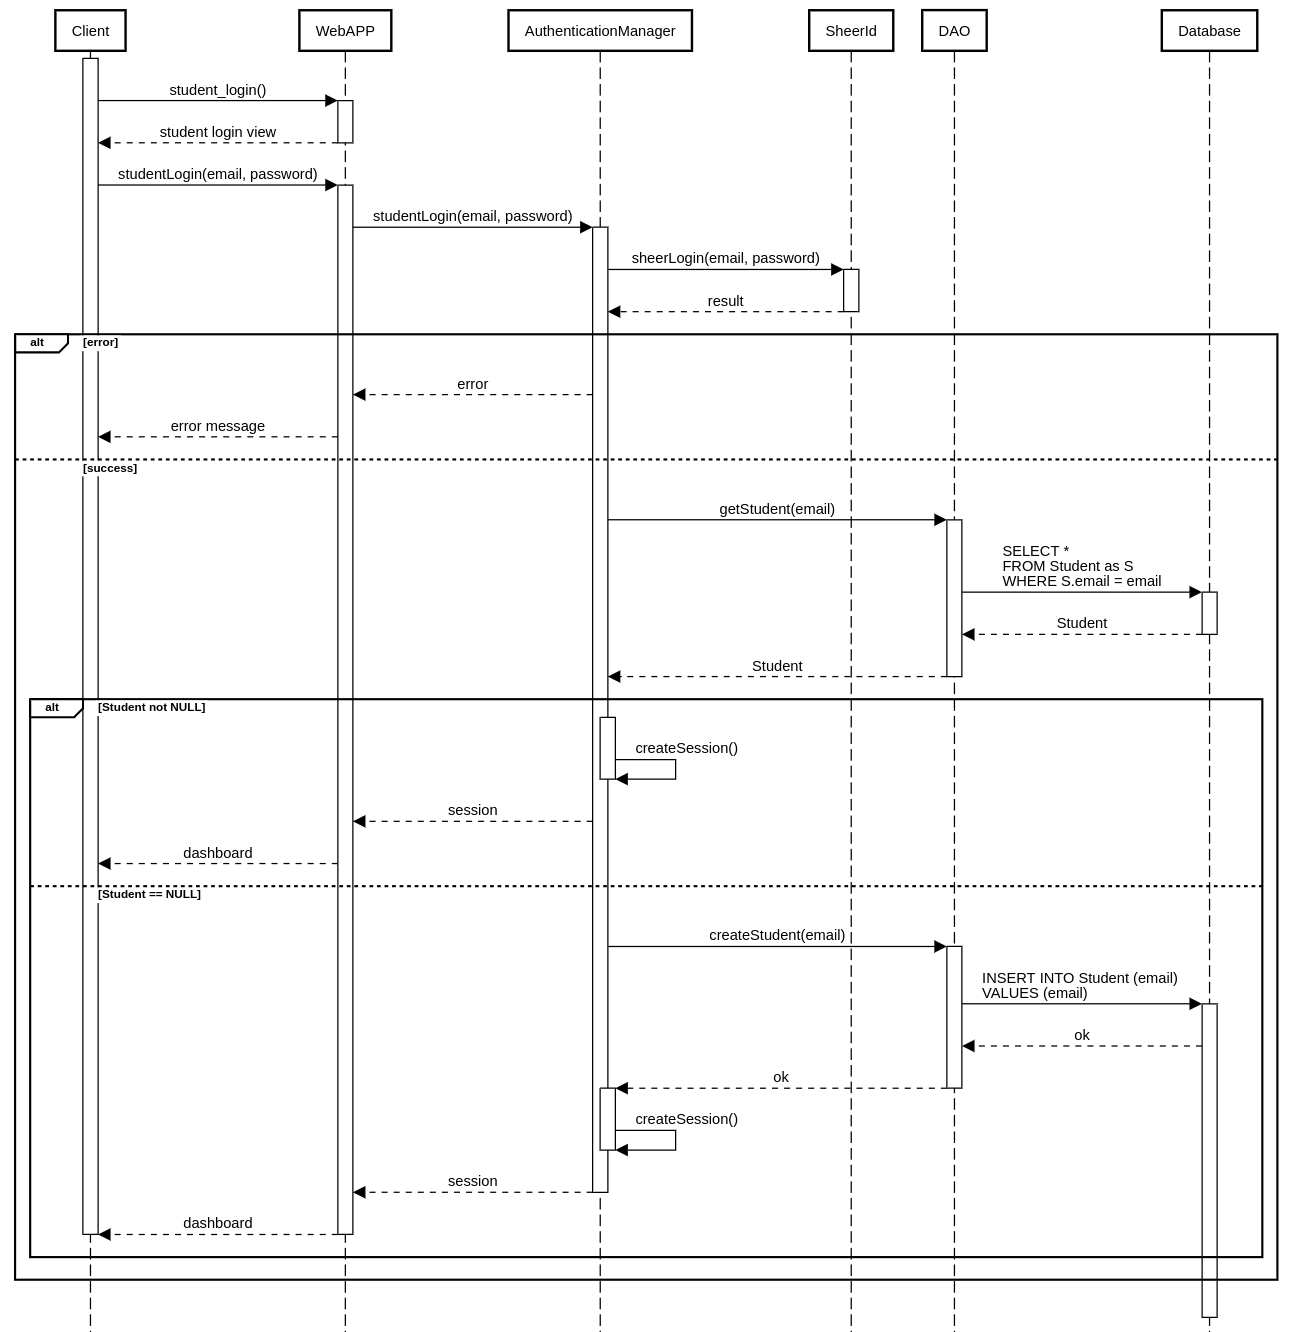
\includegraphics[width=\textwidth]{Images/UC diagrams/student_login.png}\newpage
[UC5] - Post Internship\newline
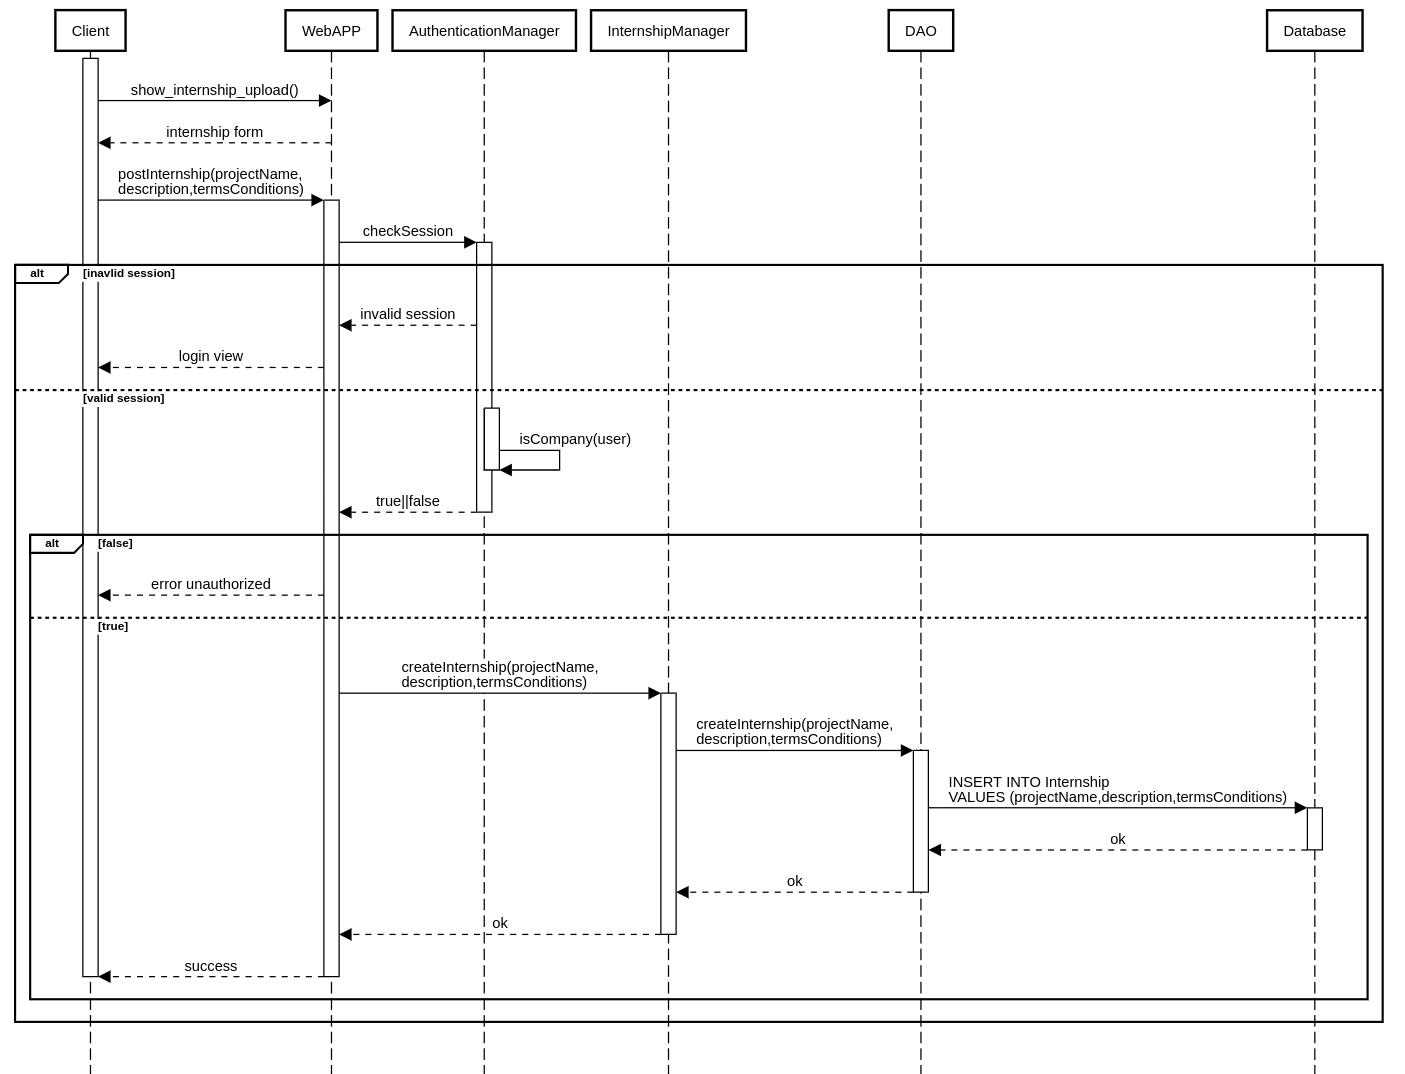
\includegraphics[width=\textwidth]{Images/UC diagrams/post_internship.png}\newpage
[UC6] - Post Feedback\newline
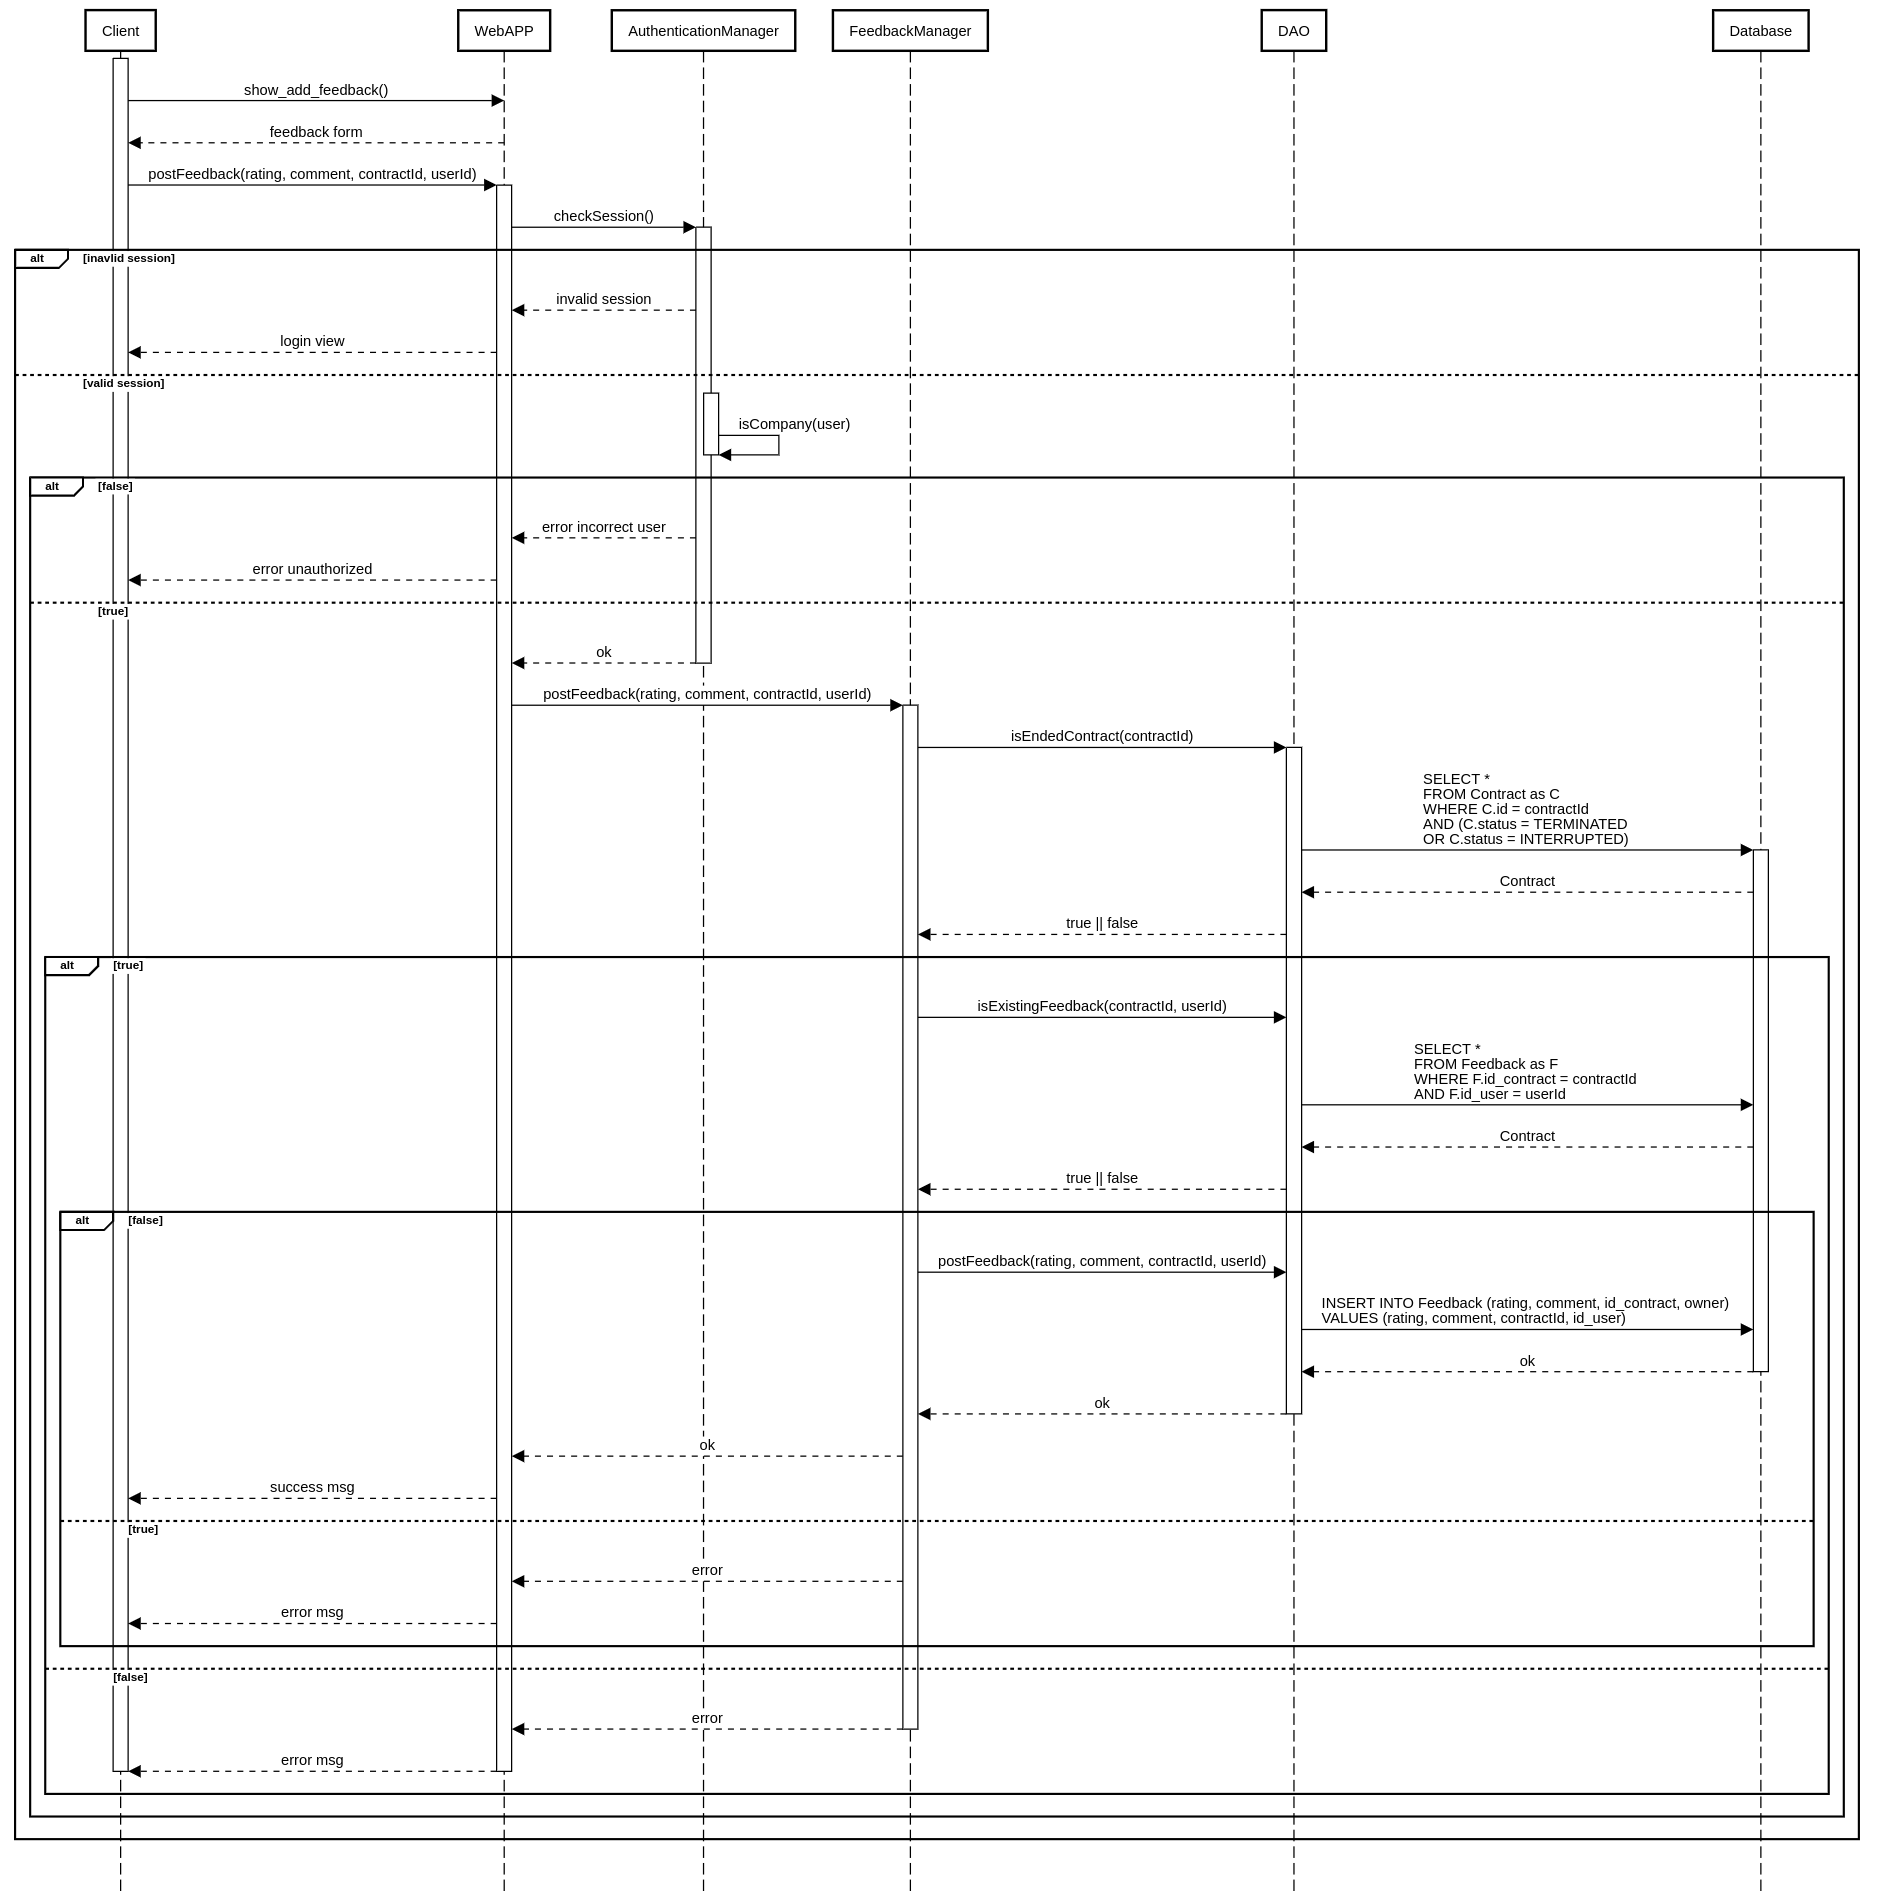
\includegraphics[width=\textwidth]{Images/UC diagrams/post_feedback.png}\newpage
[UC7] - Search Internship\newline
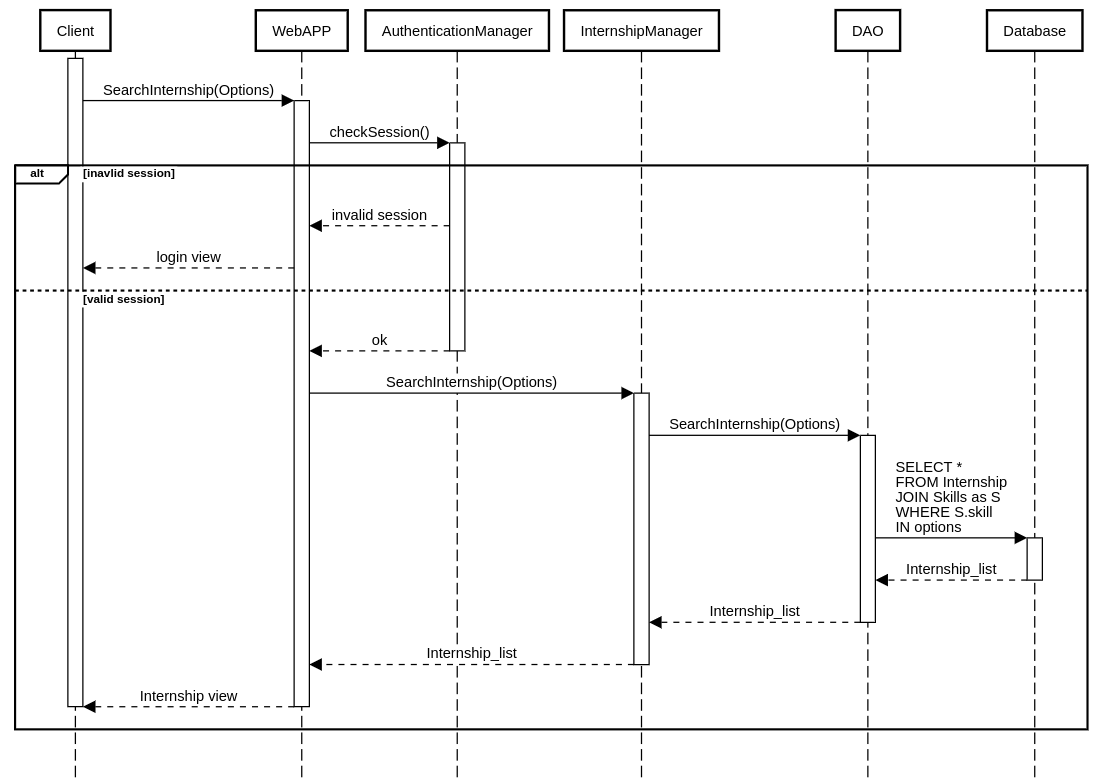
\includegraphics[width=\textwidth]{Images/UC diagrams/search_internship.png}\newpage
[UC8] - Apply for an Internship\newline
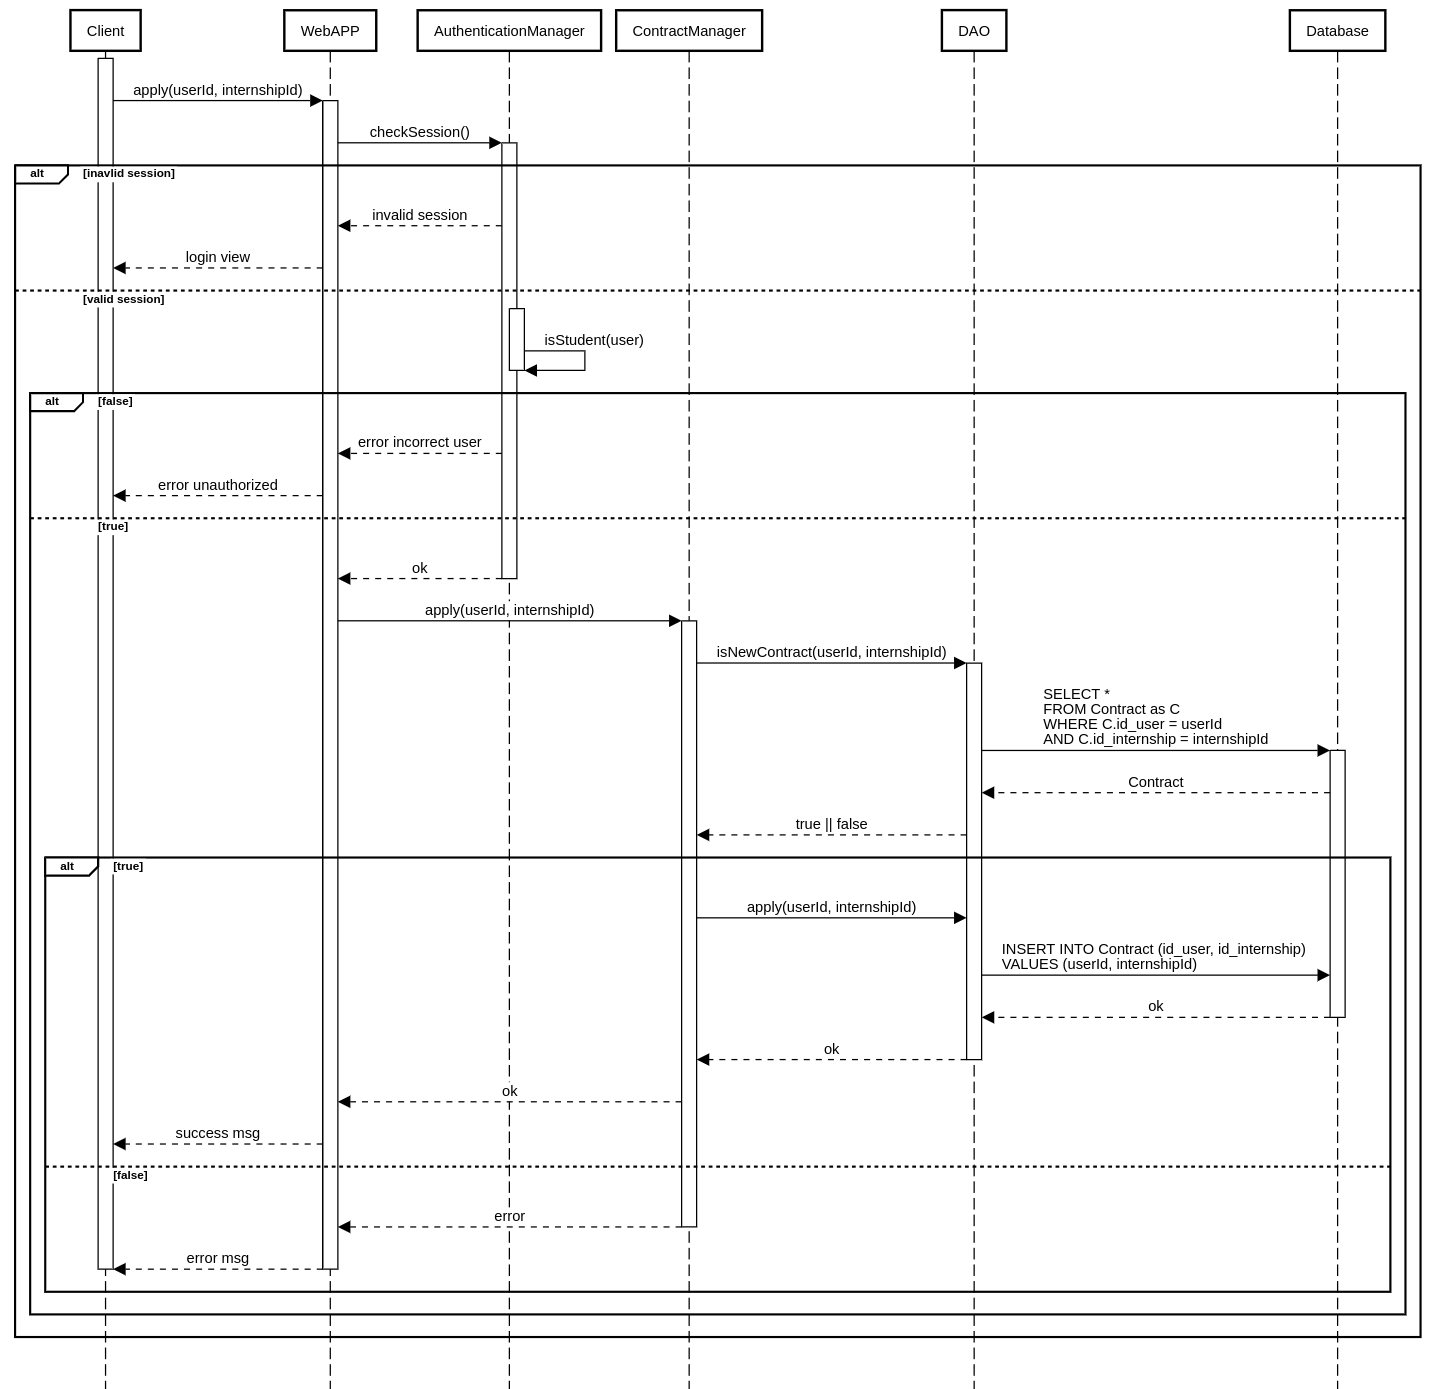
\includegraphics[width=\textwidth]{Images/UC diagrams/apply_internship.png}\newpage
[UC9] - Questionnaire Creation\newline
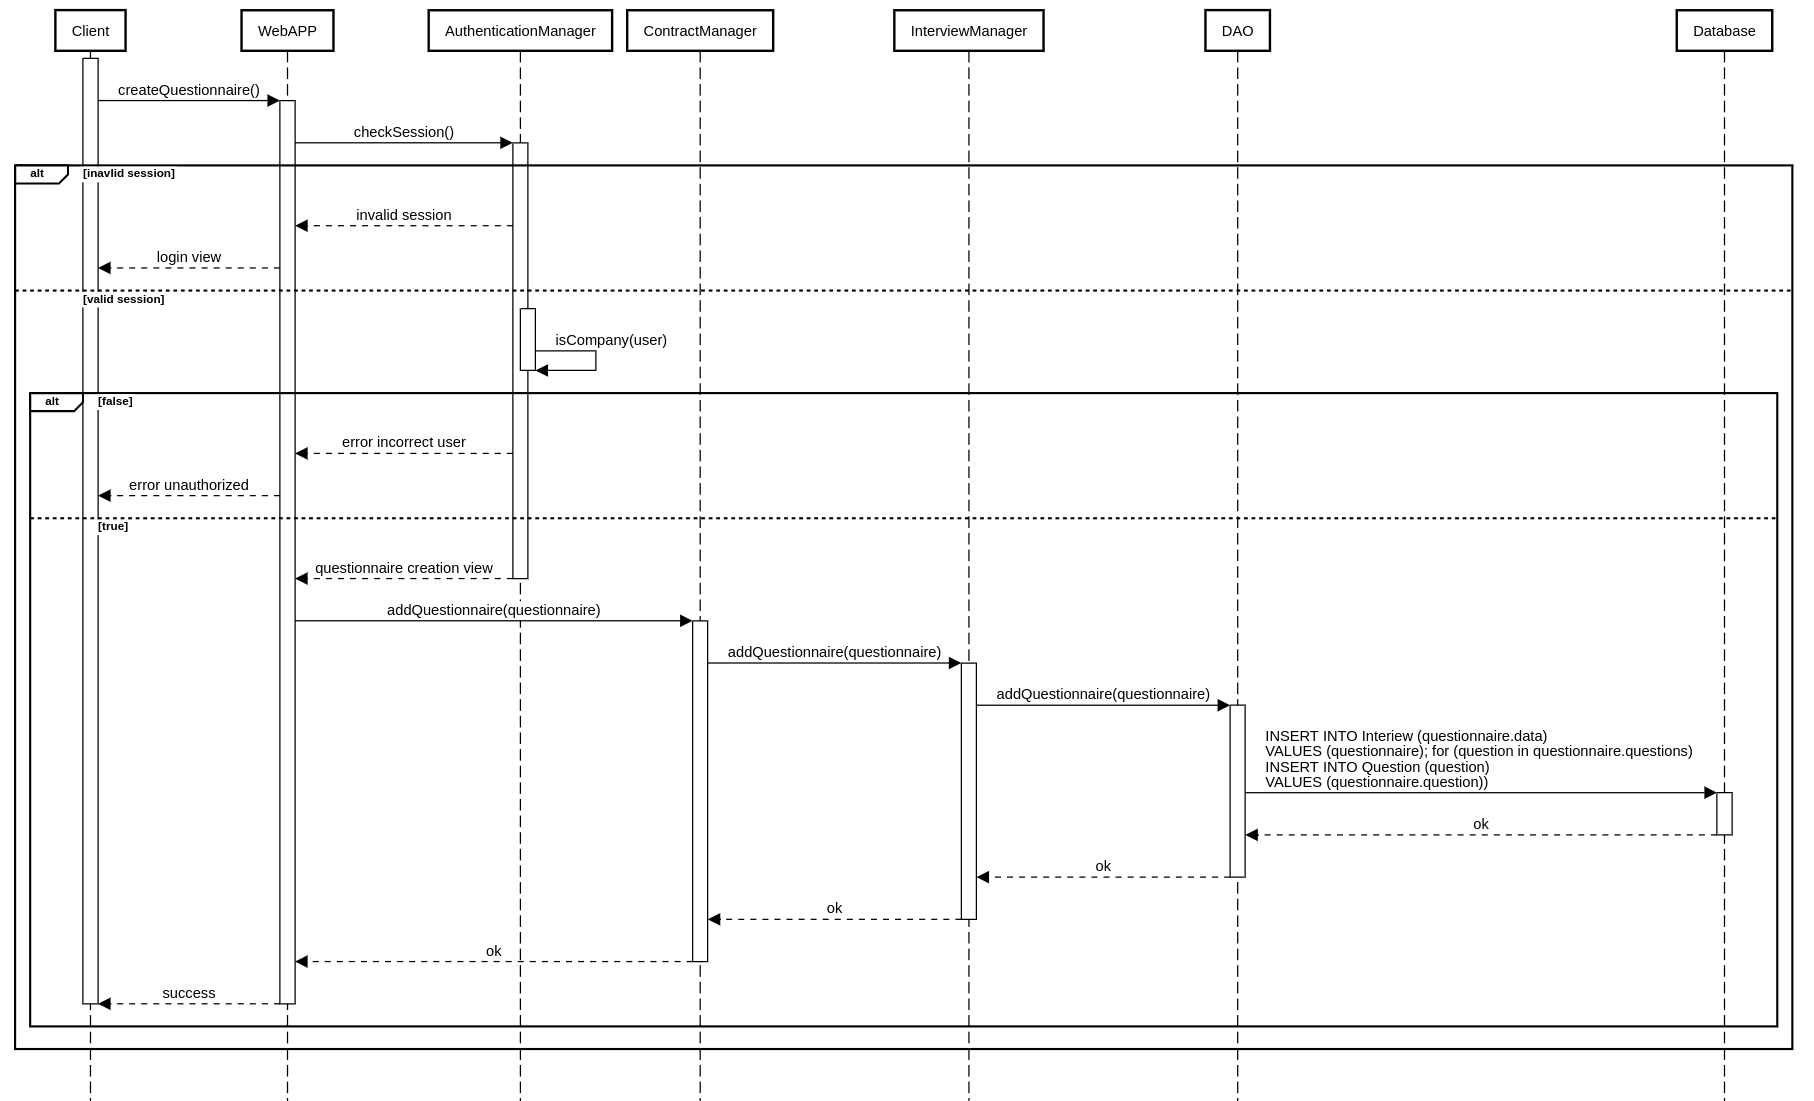
\includegraphics[width=\textwidth]{Images/UC diagrams/questionnaire_creation.png}\newpage
[UC10] - Answer Questionnaire Interview\newline
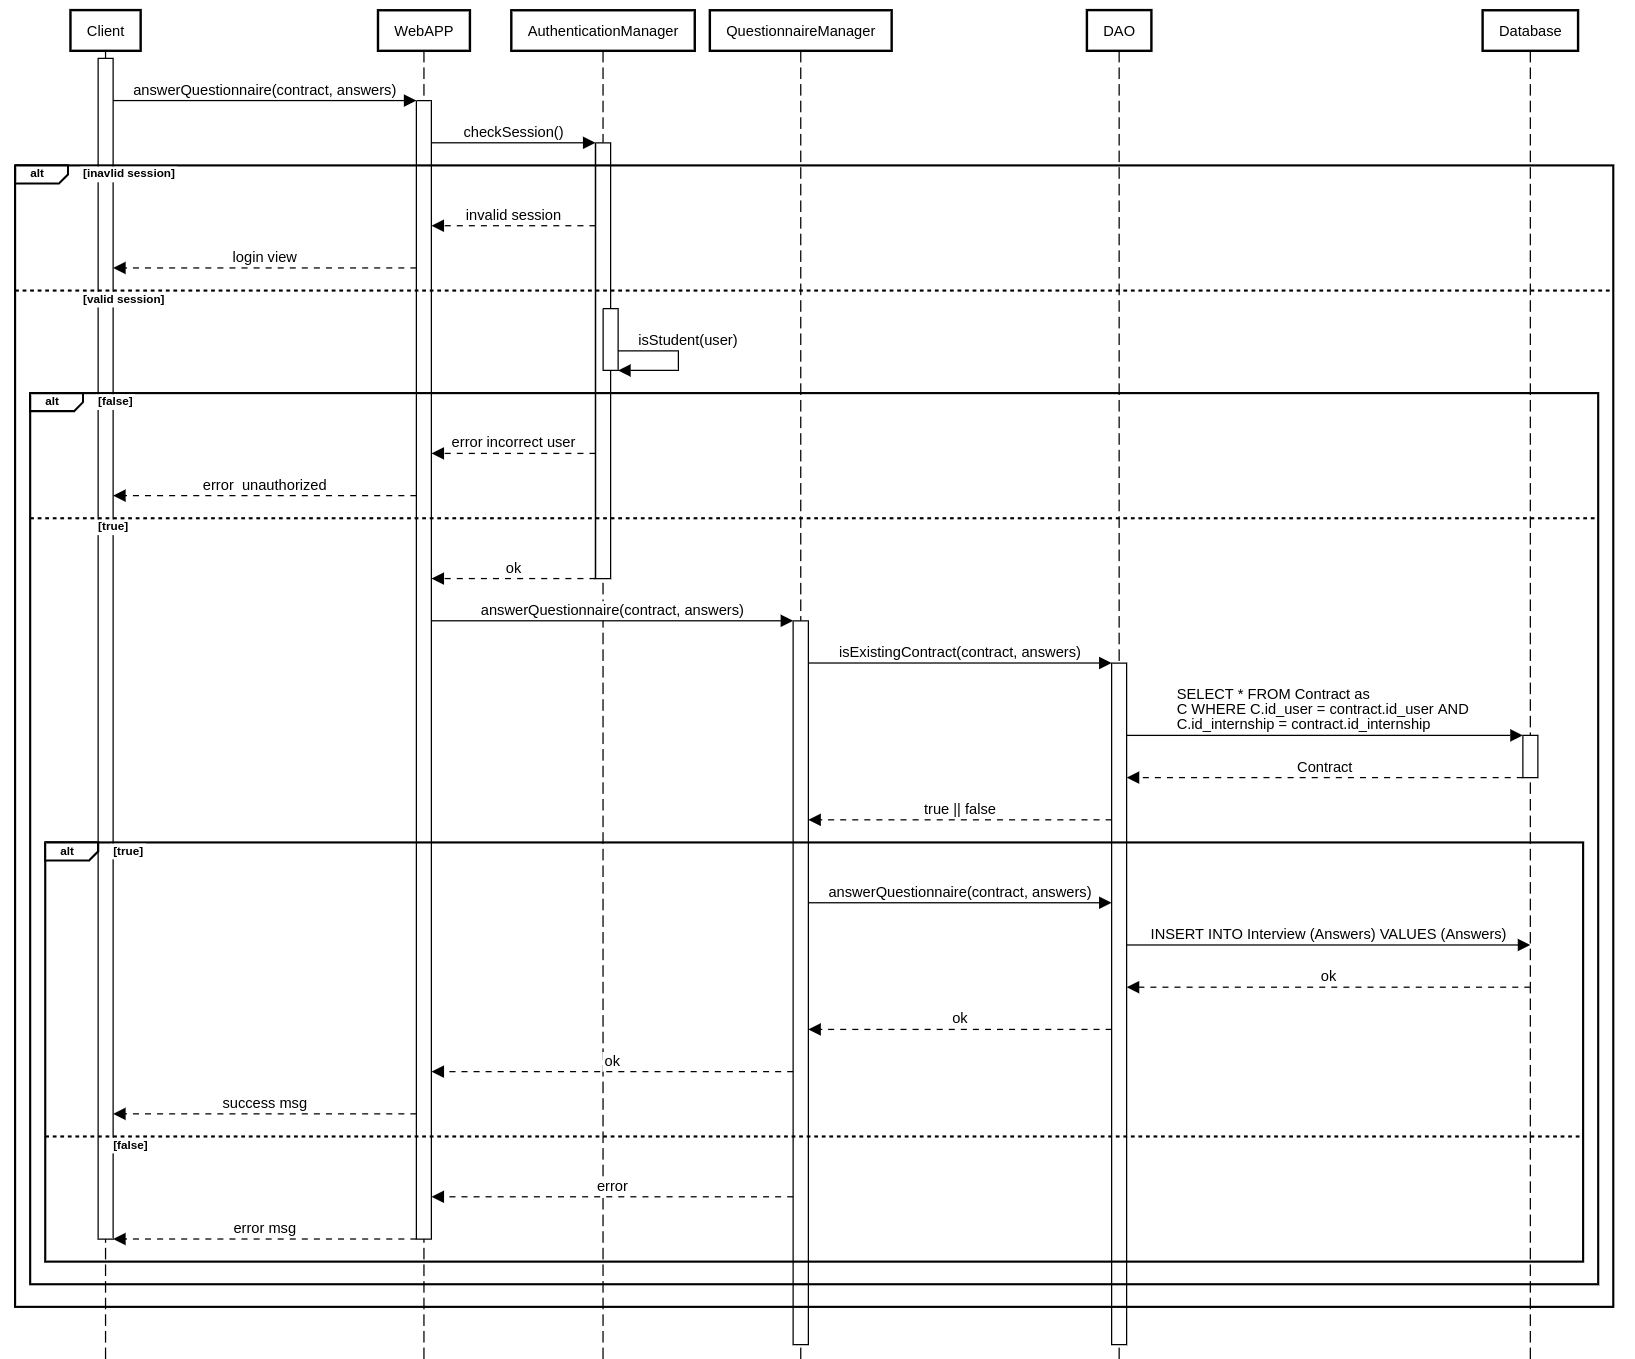
\includegraphics[width=\textwidth]{Images/UC diagrams/answer_questionnaire.png}\newpage
[UC11] - Sign Contract\newline
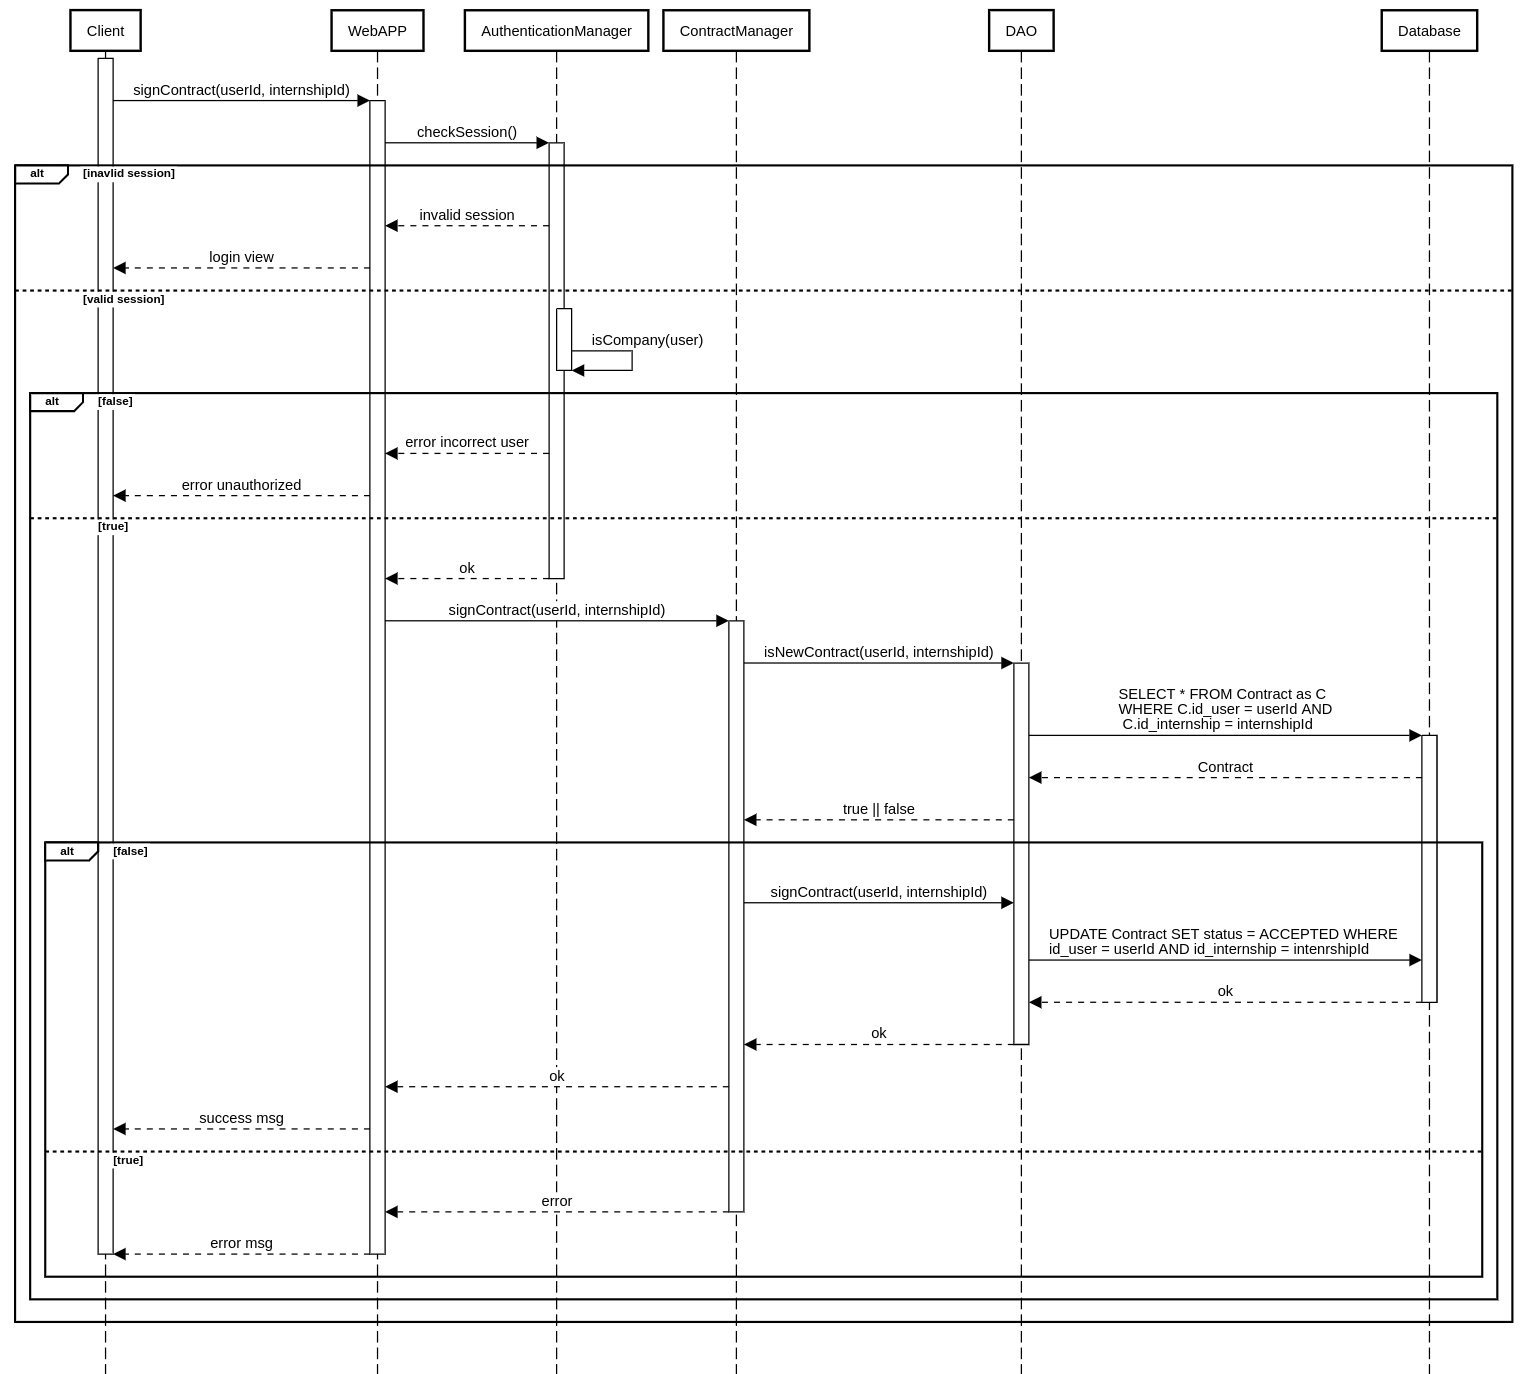
\includegraphics[width=\textwidth]{Images/UC diagrams/sign_contract.png}\newpage
[UC12] - Open Discussion\newline
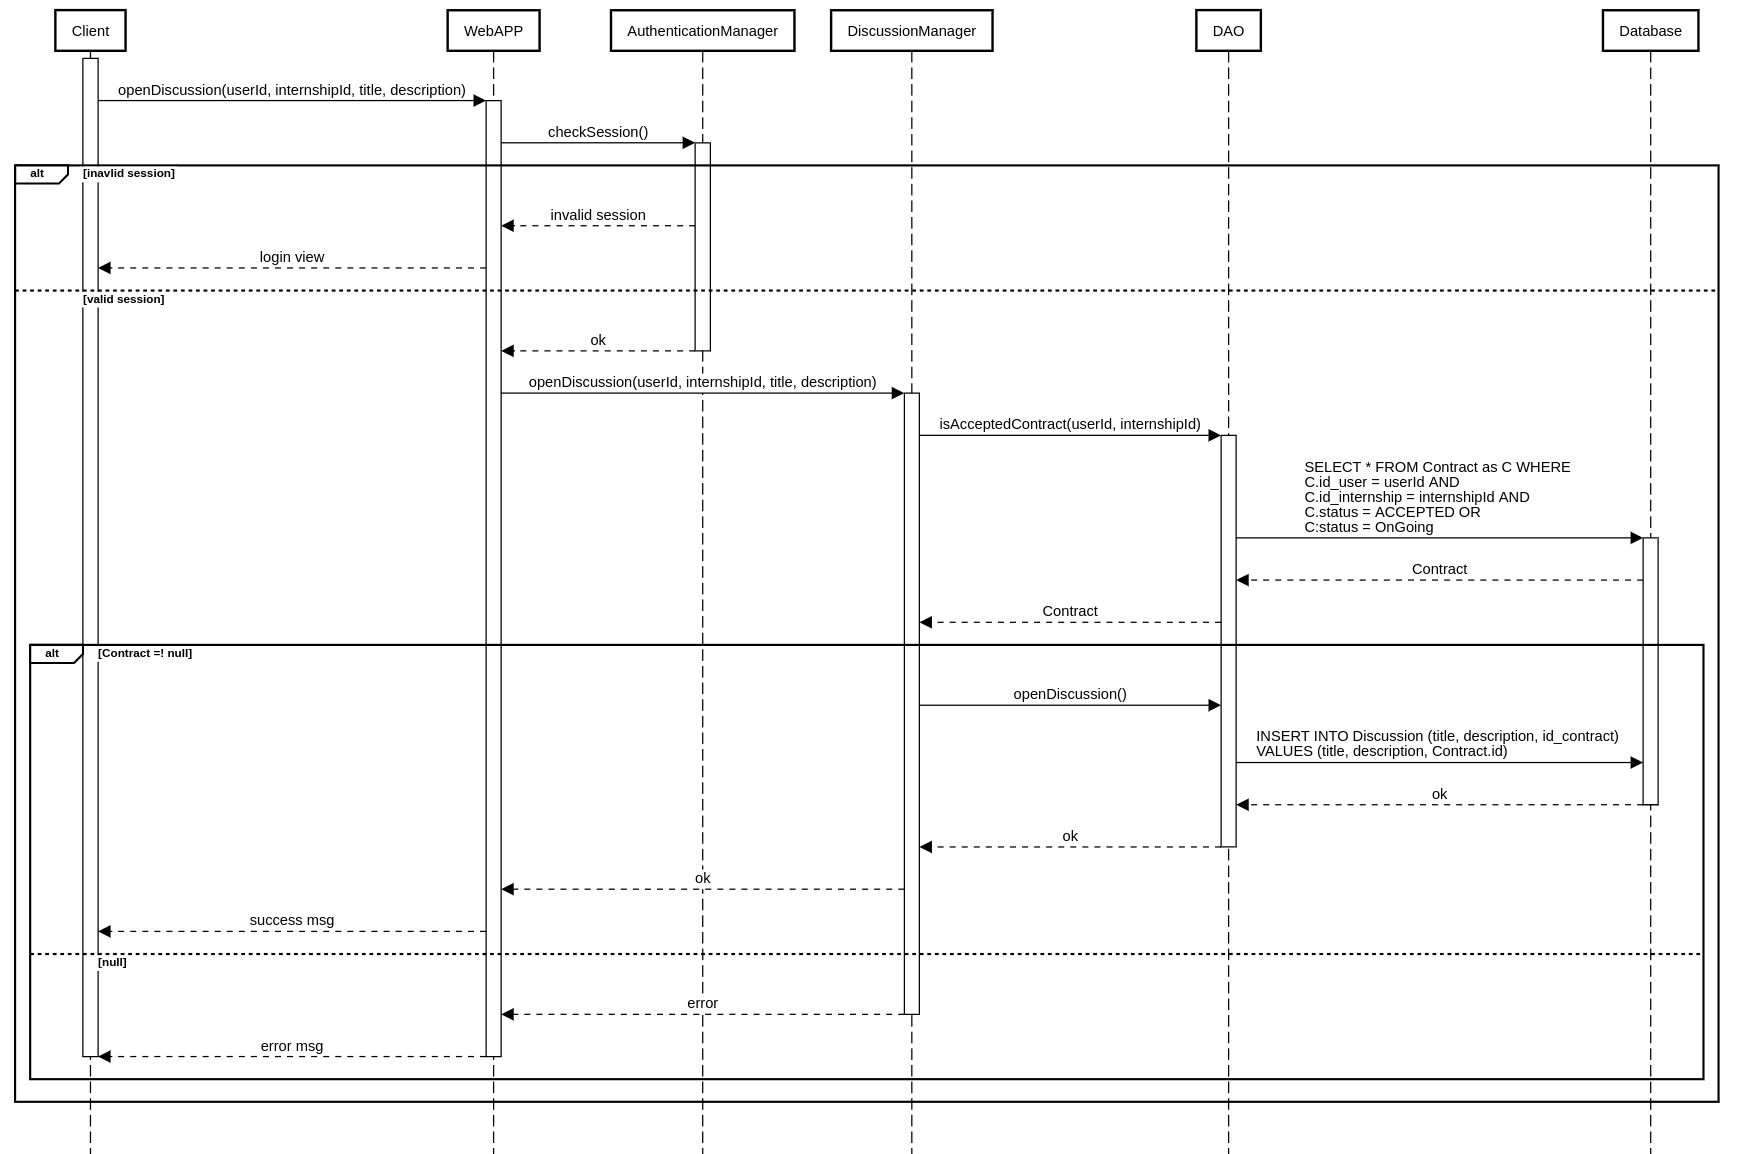
\includegraphics[width=\textwidth]{Images/UC diagrams/open_discussion.png}\newline
[UC13] - Send Message in a Discussion\newline
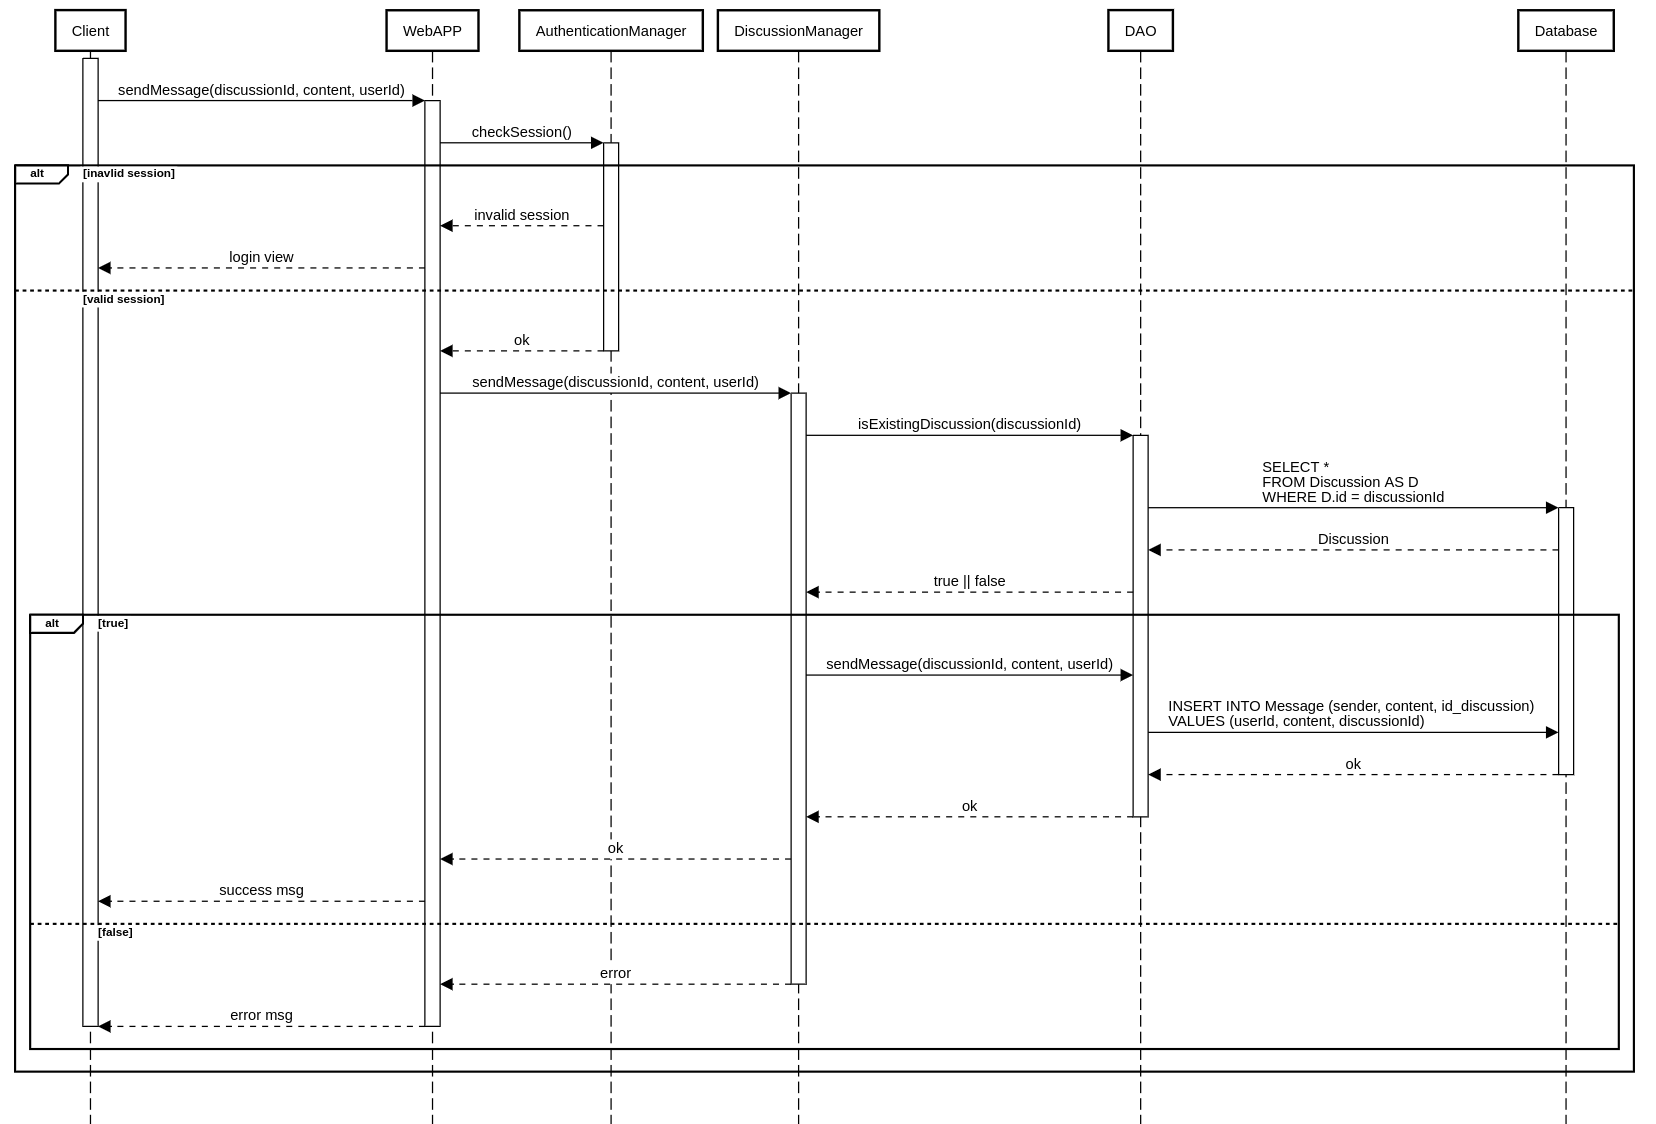
\includegraphics[width=\textwidth]{Images/UC diagrams/send_message.png}\newpage
[UC14] - Terminate Internship\newline
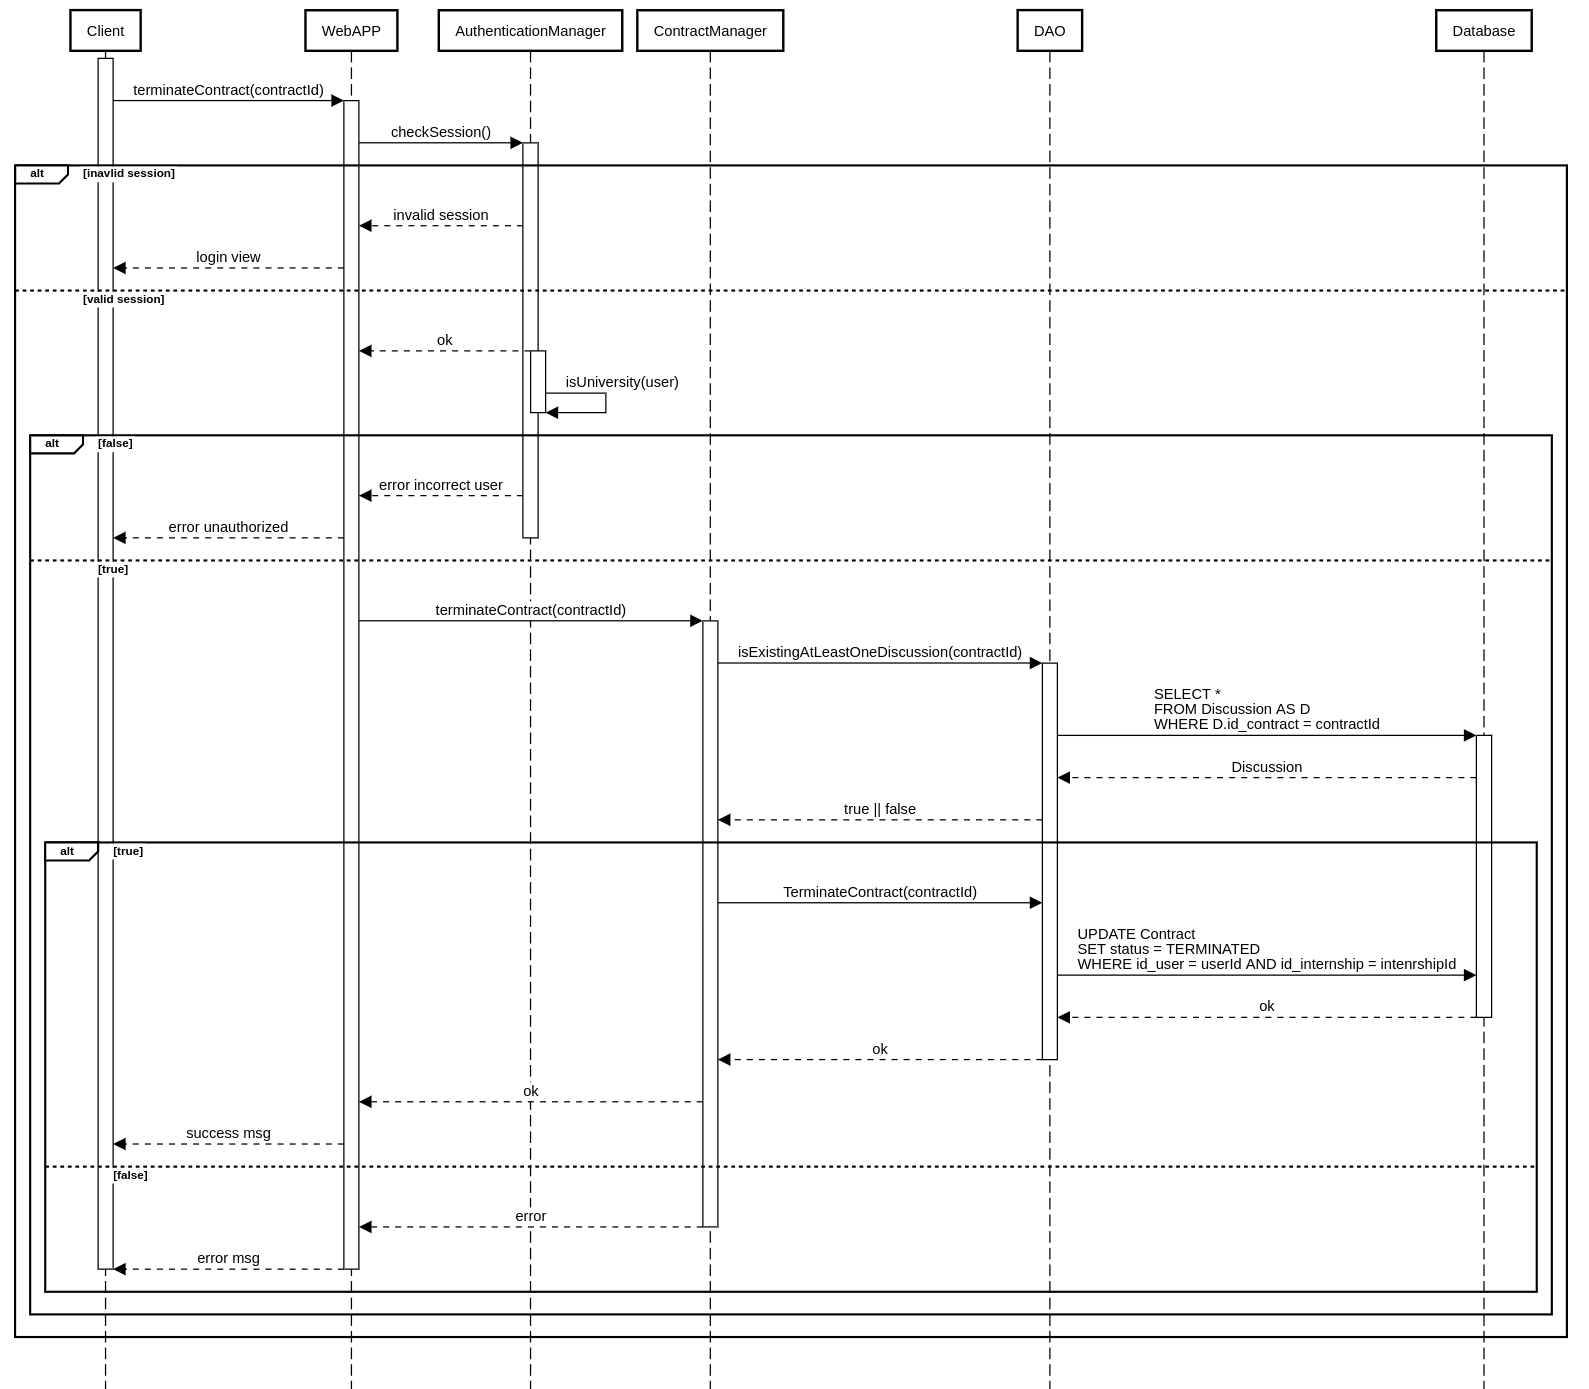
\includegraphics[width=\textwidth]{Images/UC diagrams/terminate_internship.png}\newline
[UC15] - Generate CV Improvement Suggestion\newline
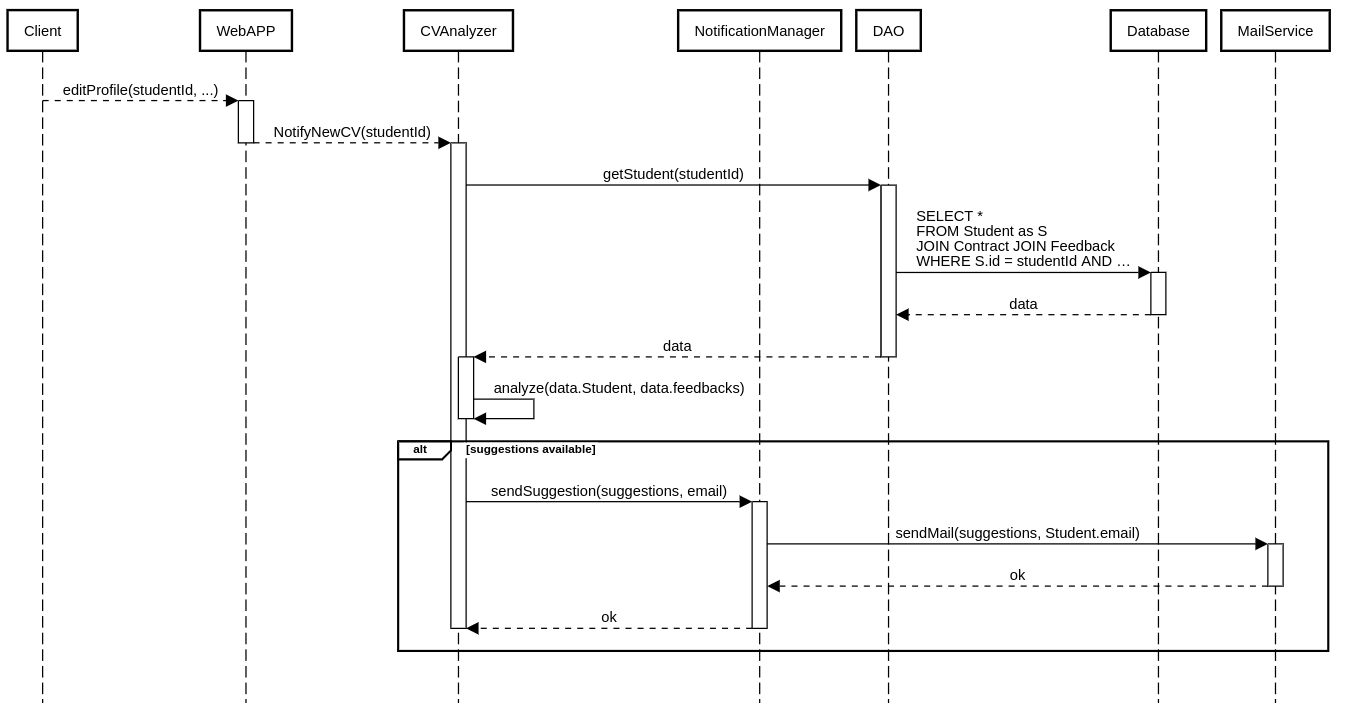
\includegraphics[width=\textwidth]{Images/UC diagrams/cv_suggestion.png}\newpage
[UC16] - Generate Internship Improvement Suggestion\newline
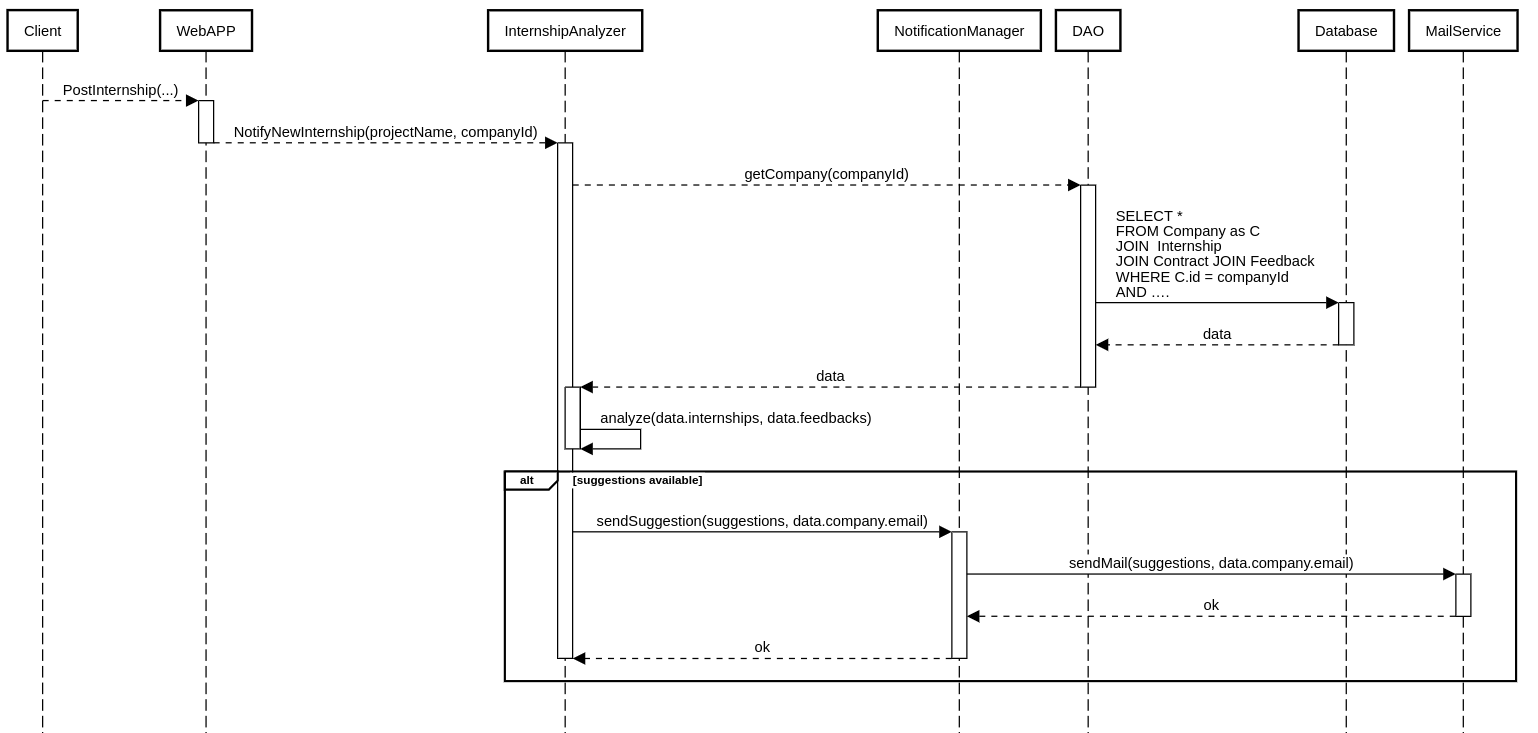
\includegraphics[width=\textwidth]{Images/UC diagrams/internship_suggestion.png}\newline
[UC17] - Student Recommendation\newline
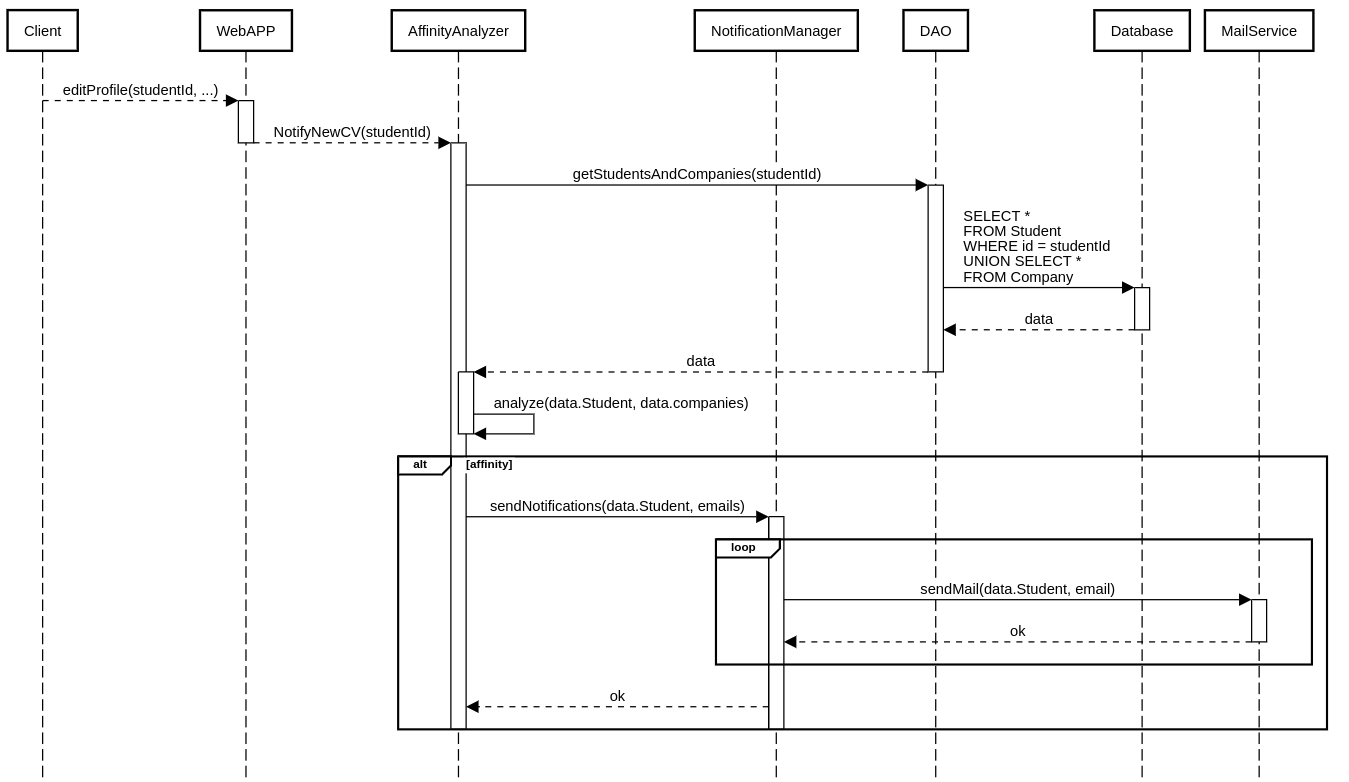
\includegraphics[width=\textwidth]{Images/UC diagrams/student_recommendation.png}\newpage
[UC18] - Internship Recommendation\newline
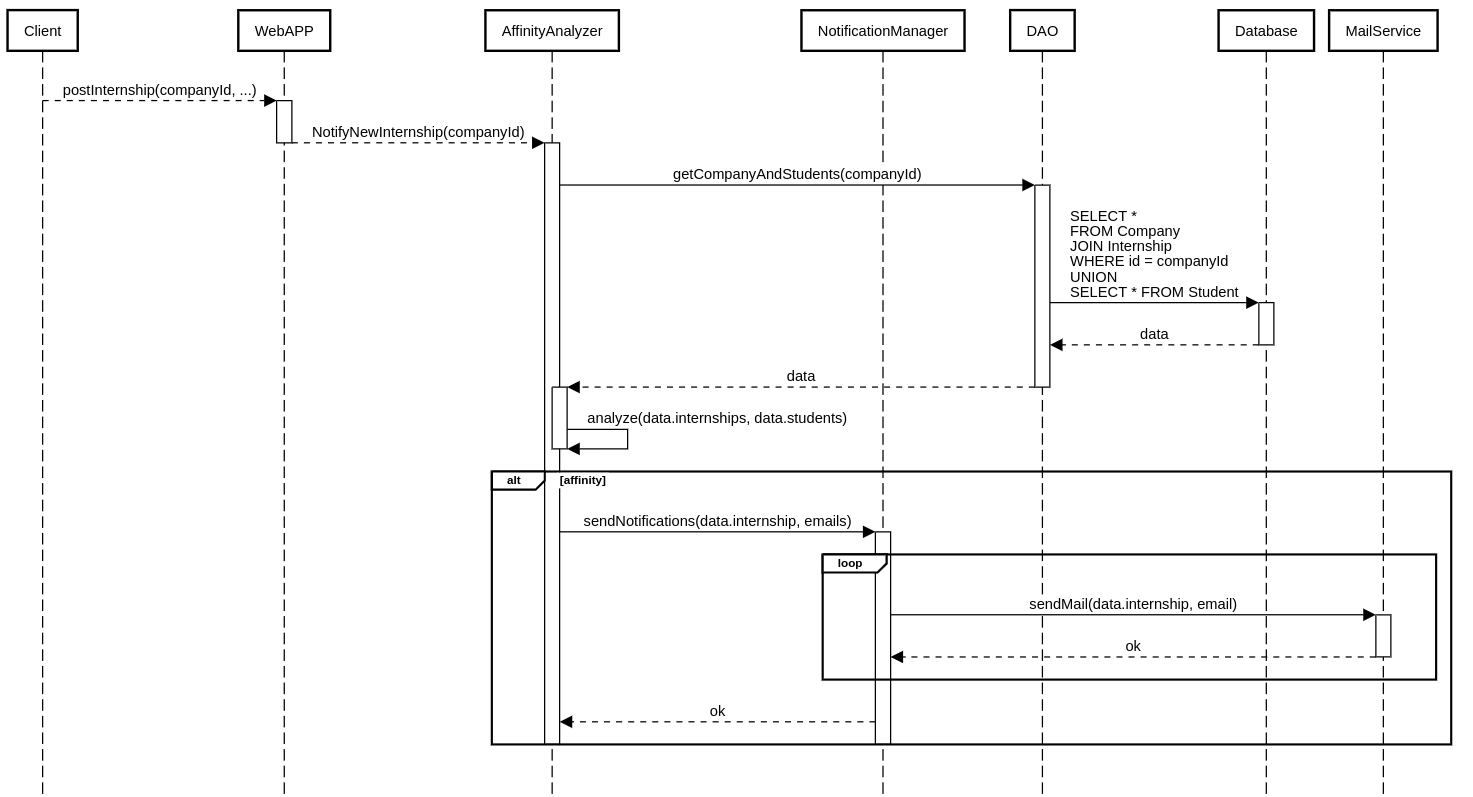
\includegraphics[width=\textwidth]{Images/UC diagrams/internship_recommendation.png}\newline
[UC19] - Monitor Internship Status\newline
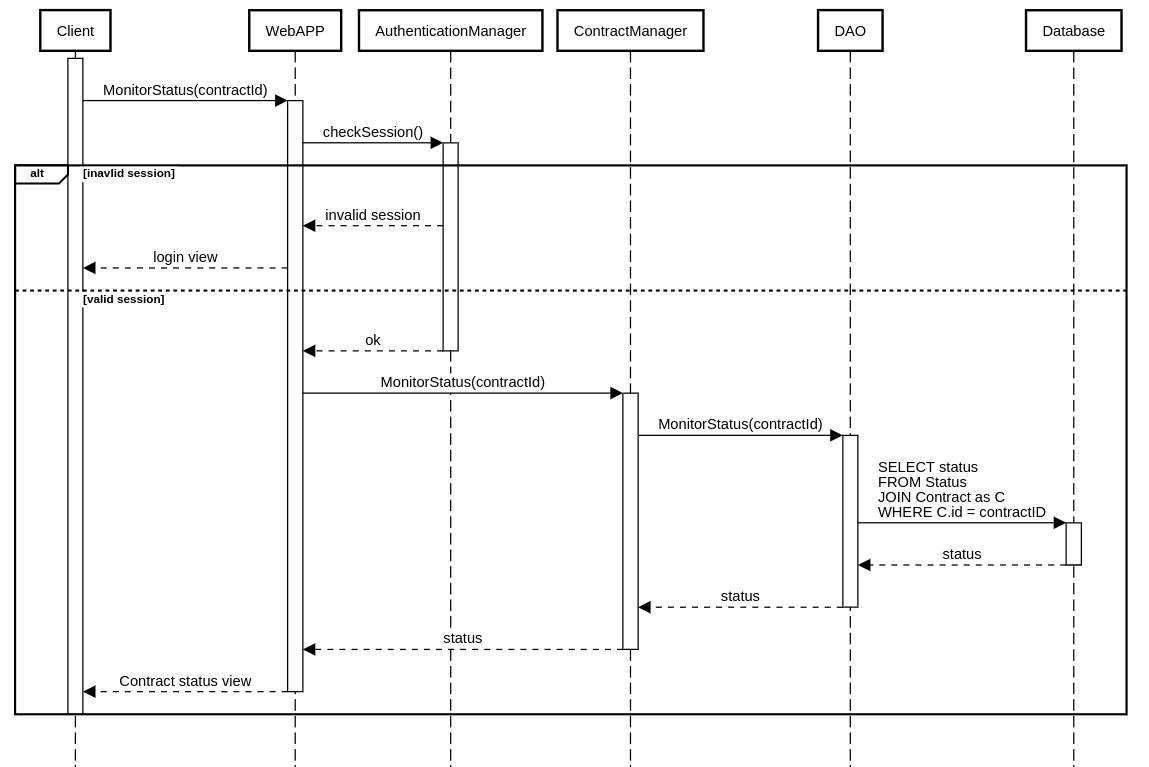
\includegraphics[width=\textwidth]{Images/UC diagrams/monitor_status.png}\newpage
[UC20] - Edit Profile\newline
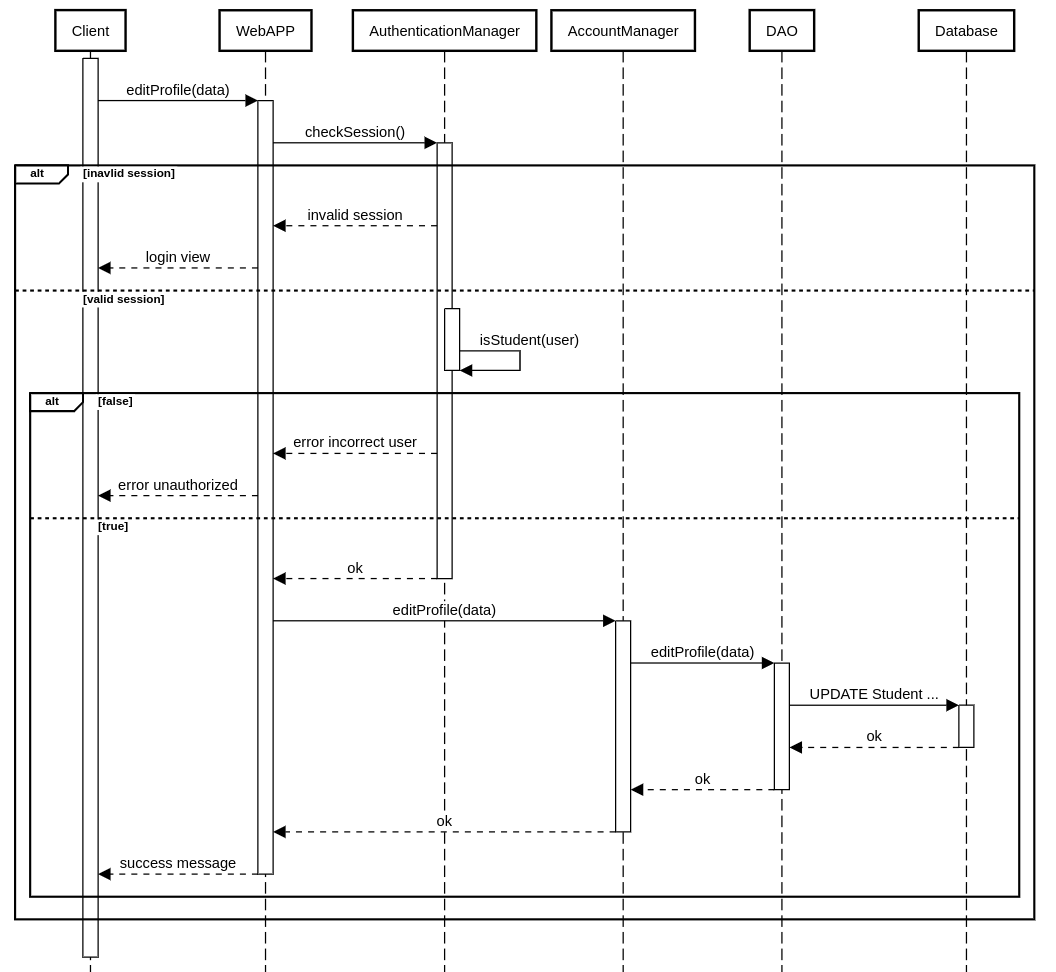
\includegraphics[width=\textwidth]{Images/UC diagrams/edit_profile.png}\newline









\subsection{Component Interfaces}
\subsubsection{WebAPP}
\begin{itemize}
    \item void: companyRegister.onClick()
    \item void: companyRegister(name, email, password, VAT)
    \item void: companyLogin.onClick()
    \item void: companyLogin(username, password)
    \item void: universityLogin.onClick()
    \item void: universityLogin(email, password)
    \item void: studentLogin.onClick()
    \item void: studentLogin(email, password)
    \item void: postInternship(projectName, description, termsConditions)
    \item void: postFeedback(rating, comment, contractId, userId)
    \item void: searchInternship(Options)
    \item void: apply(userId, internshipId)
    \item void: createQuestionnaire()
    \item void: answerQuestionnaire(contract, answers)
    \item void: signContract(userId, internshipId)
    \item void: openDiscussion(userId, internshipId, title, description)
    \item void: sendMessage(discussionId, content, userId)
    \item void: terminateContract(contractId)
    \item void: createQuestionnaire()
    \item void: monitorStatus(contractId)
\end{itemize}
\subsubsection{SheerID}
\begin{itemize}
    \item bool: SheerLogin(email, password)
\end{itemize}
\subsubsection{Database}
\begin{itemize}
    \item SELECT ...
    \item INSERT ...
    \item UPDATE ...
\end{itemize}
\subsubsection{DAO}
\begin{itemize}
    \item bool: isNewCompany(VAT)
    \item bool: isEndedContract(contractId)
    \item bool: isExistingFeedback(contractId, userId)
    \item bool: isExistingDiscussion(discussionId)
    \item bool: isAcceptedContract(userId, internshipId)
    \item bool: isExistingContract(contract, answers)
    \item bool: companyRegister(name, email, password, VAT)
    \item bool: companyLogin(username, password)
    \item bool: universityLogin(email, password)
    \item Student: getStudent(email)
    \item bool: createStudent(email, password)
    \item bool: postInternship(projectName, description, termsConditions)
    \item bool: postFeedback(rating, comment, contractId, userId)
    \item List<Internship>: SearchInternship(Options)
    \item bool: apply(userId, internshipId)
    \item bool: createQuestionnaire()
    \item bool: answerQuestionnaire(contract, answers)
    \item bool: signContract(userId, internshipId)
    \item bool: openDiscussion(userId, internshipId, title, description)
    \item bool: sendMessage(discussionId, content, userId)
    \item bool: terminateContract(contractId)
    \item bool: editProfile(data)
    \item bool: addQuestionnaire(questionnaire)
    \item STATUS: monitorStatus(contractId)
\end{itemize}
\subsubsection{AuthenticationManager}
\begin{itemize}
    \item JSON: createSession()
    \item bool: checkSession()
    \item Company: companyLogin(email, password)
    \item University: universityLogin(email, password)
    \item Student: studentLogin(email, password)
    \item bool: isCompany(user)
    \item bool: isStudent(user)
    \item bool: isUniversity(user)
\end{itemize}
\subsubsection{AccountManager}
\begin{itemize}
    \item bool: companyRegister(name, email, password, VAT)
    \item bool: editProfile(data)
\end{itemize}
\subsubsection{InternshipManager}
\begin{itemize}
    \item bool: postInternship(projectName, description, termsConditions)
    \item List<Internship>: SearchInternship(Options)
\end{itemize}
\subsubsection{ContractManager}
\begin{itemize}
    \item bool: apply(userId, internshipId)
    \item bool: addQuestionnaire(questionnaire)
    \item bool: signContract(userId, internshipId)
    \item bool: terminateContract(contractId)
    \item STATUS: MonitorStatus(contractId)
\end{itemize}
\subsubsection{FeedbackManager}
\begin{itemize}
    \item bool: postFeedback(rating, comment, contractId, userId)
\end{itemize}
\subsubsection{DiscussionManager}
\begin{itemize}
    \item bool: openDiscussion(userId, internshipId, title, description)
    \item bool: sendMessage(discussionId, content, userId)
\end{itemize}
\subsubsection{InterviewManager}
\begin{itemize}
    \item bool: answerQuestionnaire(contract, answers)
\end{itemize}
\subsubsection{InternshipAnalyzer}
\begin{itemize}
    \item void: NotifyNewIntership(projectName, companyId)
    \item {bool, String, email}: analyze(internship, feedbacks)
\end{itemize}
\subsubsection{CVAnalyzer}
\begin{itemize}
    \item void: NotifyNewCV(studentId)
    \item {bool, String, email}: analyze(student, feedbacks)
\end{itemize}
\subsubsection{AffinityAnalyzer}
\begin{itemize}
    \item {bool, String, List<email>}: analyze(student, companies)
    \item {bool, String, List<email>}: analyze(internship, students)
\end{itemize}
\subsubsection{NotificationManager}
\begin{itemize}
    \item bool: sendSuggestio(suggestions, email)
    \item bool: sendNotification(data, email)
\end{itemize}
\subsubsection{MailService}
\begin{itemize}
    \item bool: sendMail(data, mail)
\end{itemize}

\subsection{Selected Architectural Styles and Patterns}
\subsubsection{3-tier Architecture}
The architecture chosen for the S\&C system is a 3-tier client-server model, with the tiers assigned to the presentation, logic, and data layers, respectively. This architecture, characterized by highly decoupled components, enables the creation of a system that is both easily maintainable and flexible, allowing different aspects to be tested and updated independently. The tiers are described in more detail below:
\begin{itemize}
    \item \textbf{Web Client}: This tier is represented by web browsers, which provide the user interface for interacting with the system.
    \item \textbf{Application Server}: This tier handles all business logic, processes requests from the web client, and generates the pages or responses to be displayed on the clients.
    \item \textbf{Database Server}: This layer is simply a database for storing persistently and providing data as needed.
\end{itemize}
\subsubsection{Model View Controller Patter}
The Model-View-Controller (MVC) pattern is a widely used architectural design that aligns closely with the principles of the 3-tier architecture. In the MVC pattern, the Model represents the underlying data and business logic, corresponding to the database server and the DAOs of the application server. The View represents the user interface, similar to the web client tier, and is responsible for presenting data to the user. Finally, the Controller, implemented using the Handlers shown above, serves as the intermediary, handling user input and updating the Model or View as necessary. This separation of concerns allows for modular design, facilitating maintainability, scalability, and ease of testing, making the MVC pattern a natural fit for modern web and software applications.
\subsubsection{RESTful API}
The communication between client and server is handled through a REST API. This way, queries are HTTP based and can have an additional level of security using SSL encryption with HTTPS. Moreover REST has caching capabilities, enhancing performance even at scale since requests can be resolved directly by the client. Another advantage over other communication styles is statelessness which leads to naturally independent requests that can be handled concurrently.
\subsection{Other Design Decisions}
\subsubsection{Load Balancer}
A fundamental component in the system’s architecture is the load balancer. This device distributes incoming requests between the replicated application servers to avoid overloads resulting in increased response times and to seamlessly add (or remove) servers as needed. Load balancers can also protect the system from DDOS attacks, rate limiting clients issuing requests too frequently.

\clearpage
{\color{Blue}{\section{User Interface Design}}}
\label{sect:ui}
Initial Page\\\\
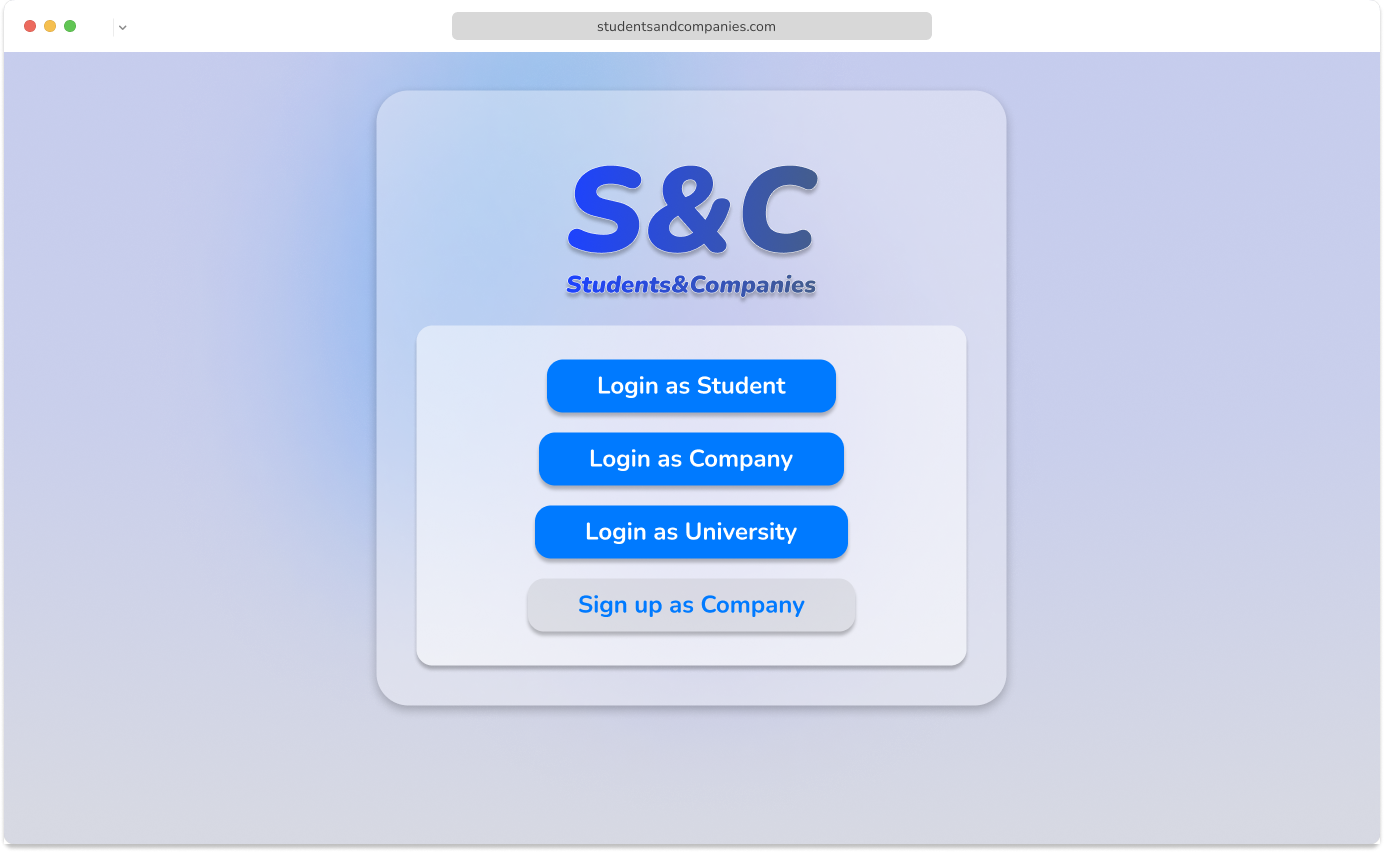
\includegraphics[width=\textwidth]{Images/MockUps/initial.png}\\\\
User Login\\\\
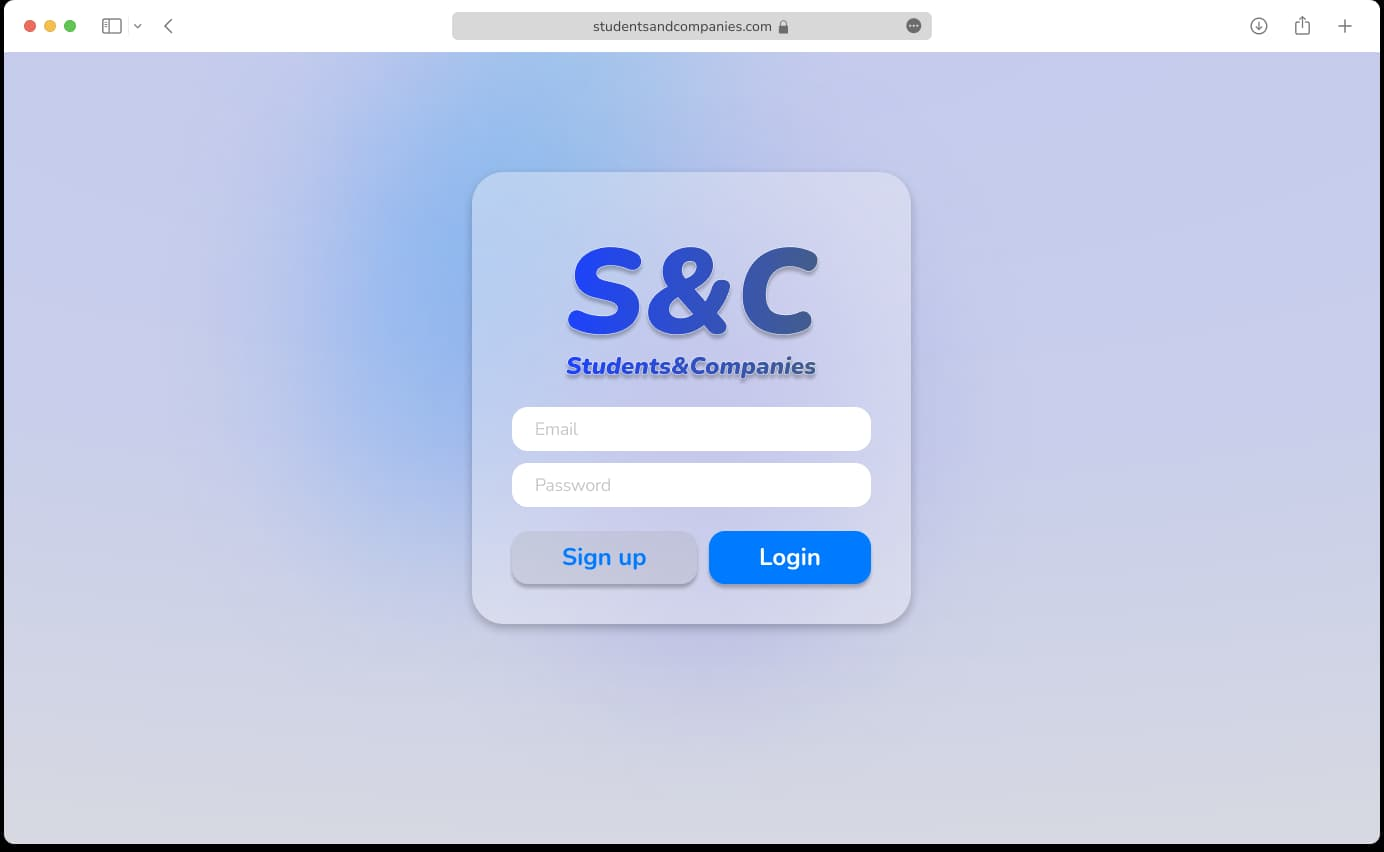
\includegraphics[width=\textwidth]{Images/MockUps/login.jpeg}\\\\
The login window varies for each user type. Additionally, the registration button is visible only when the 'login as company' button has been clicked.\\\\
Edit Profile\\\\
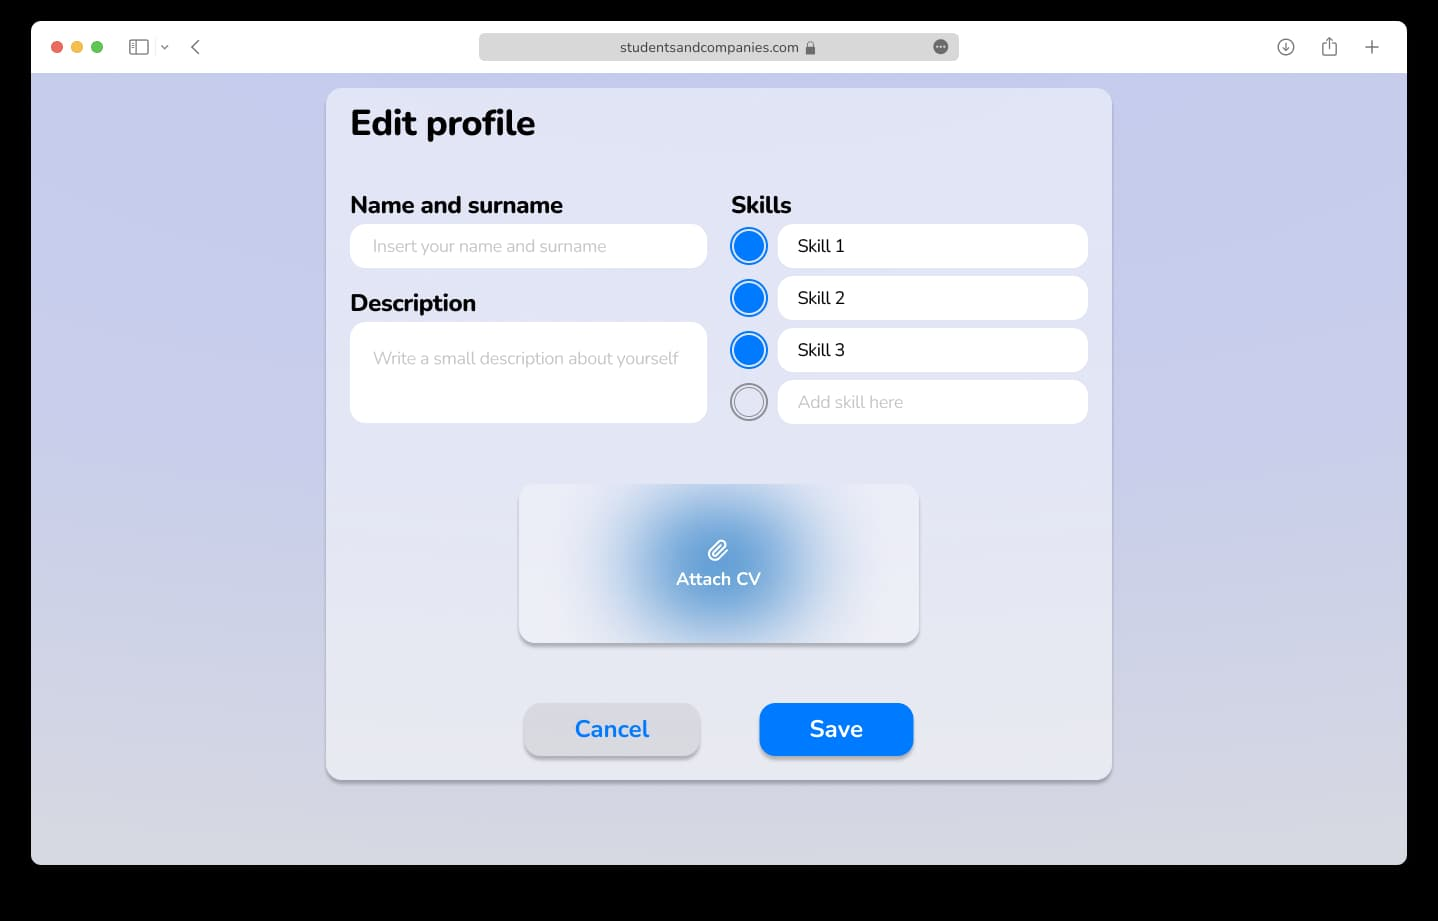
\includegraphics[width=\textwidth]{Images/MockUps/edit_profile.jpeg}\\\\
Search Internship\\\\
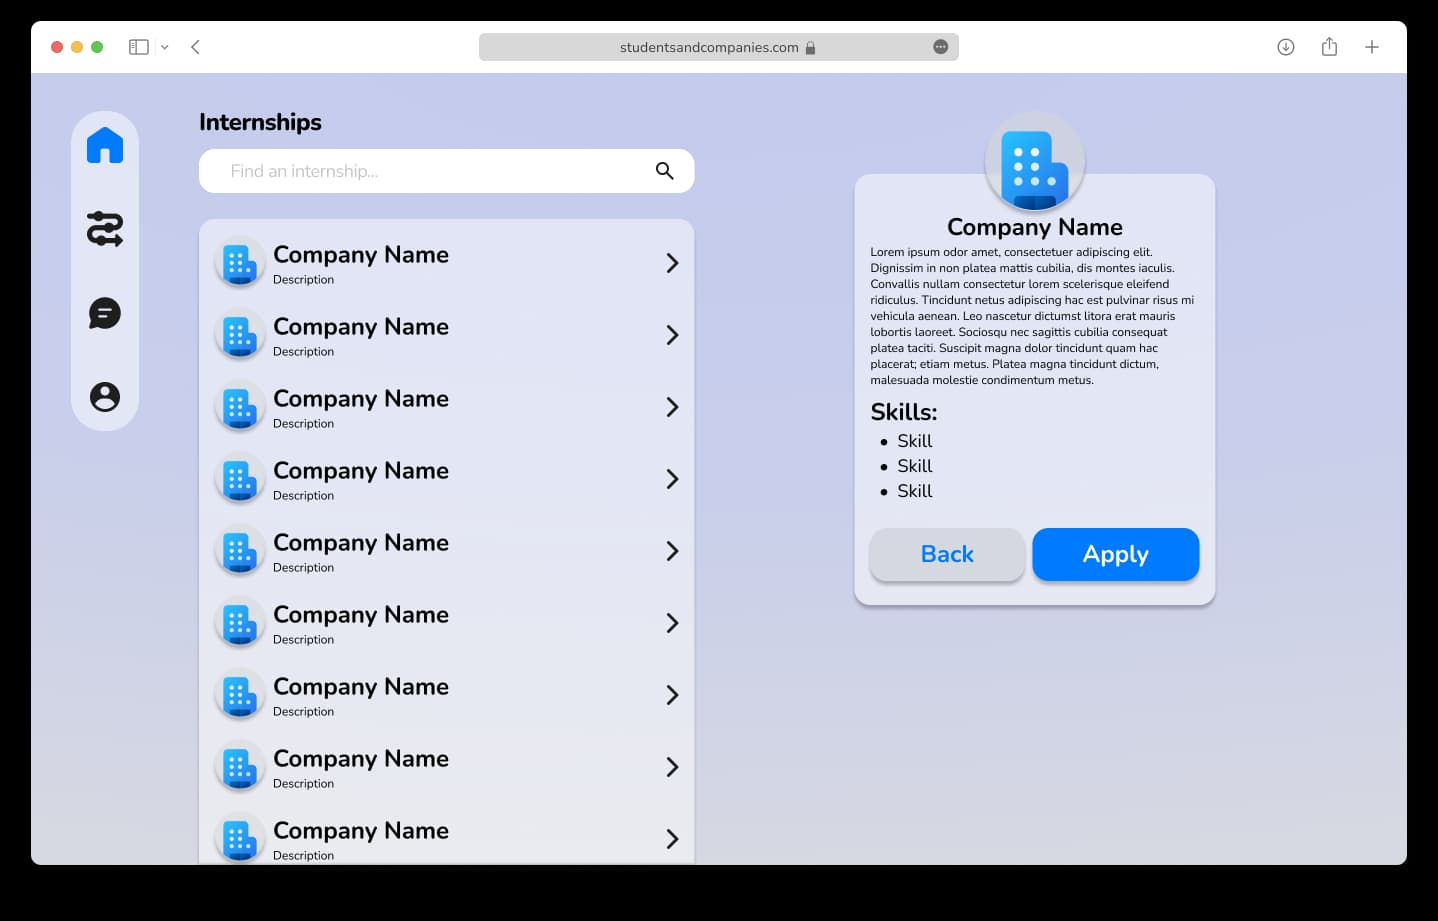
\includegraphics[width=\textwidth]{Images/MockUps/search_internship.jpeg}\\\\
Create Questionnaire\\
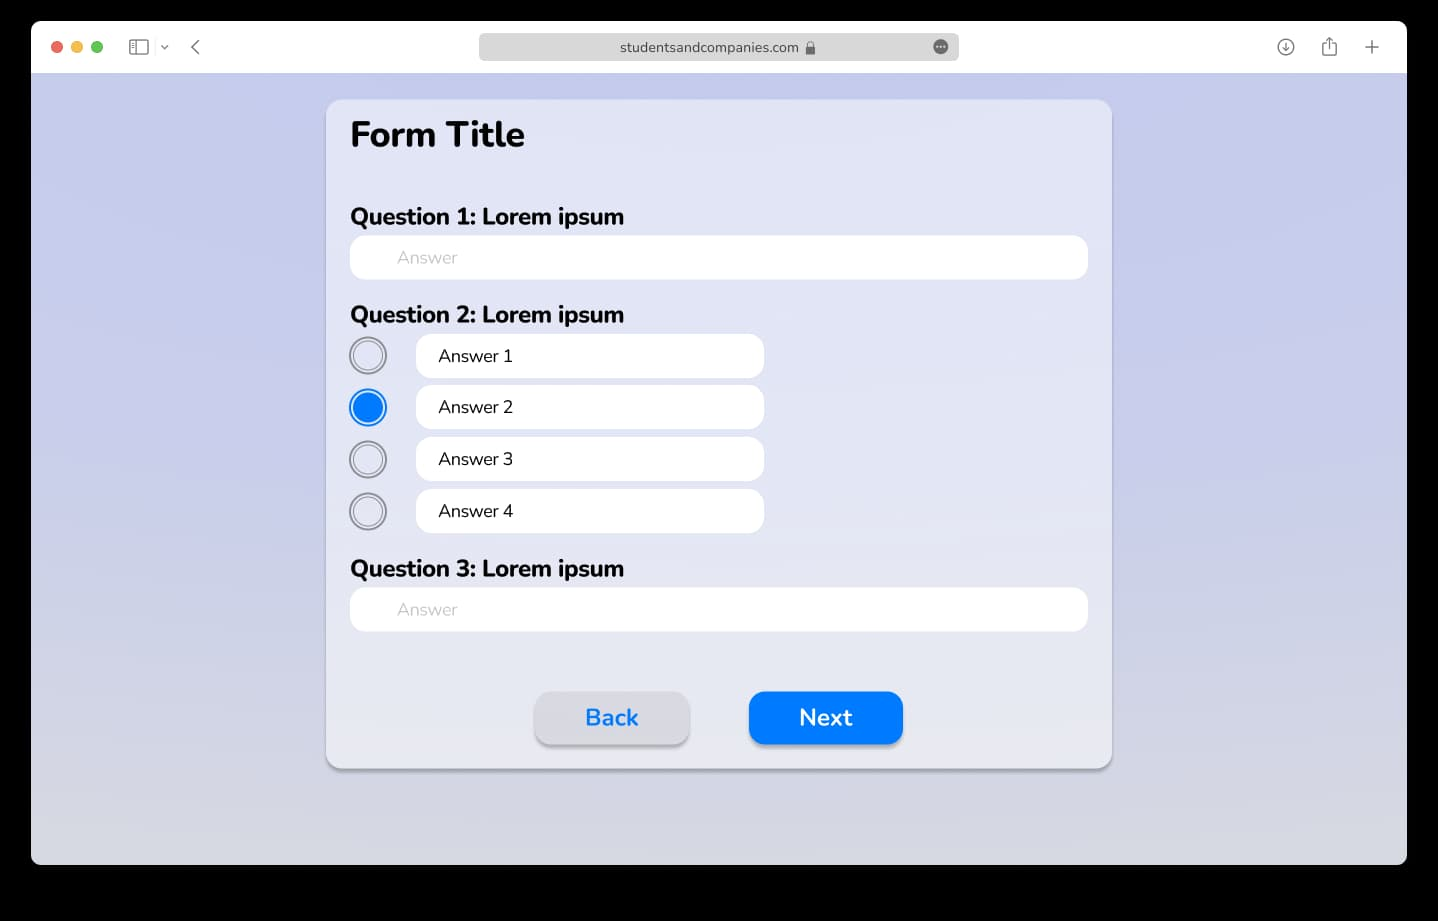
\includegraphics[width=\textwidth]{Images/MockUps/create_questionnaire.jpeg}\\\\
Discussion\\\\
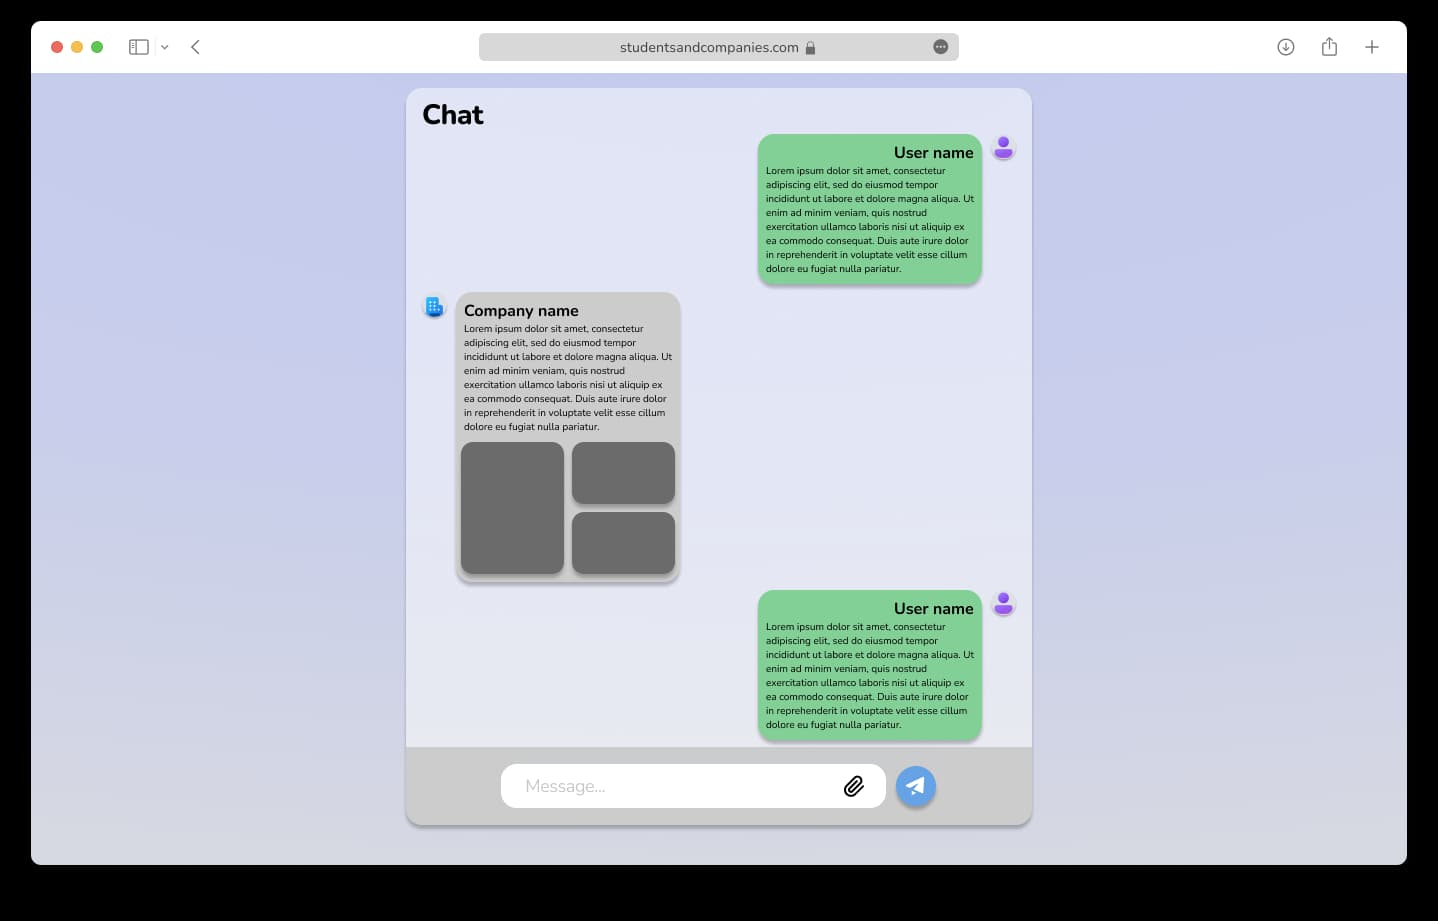
\includegraphics[width=\textwidth]{Images/MockUps/discussion.jpeg}\\\\
Upload Internship\\\\
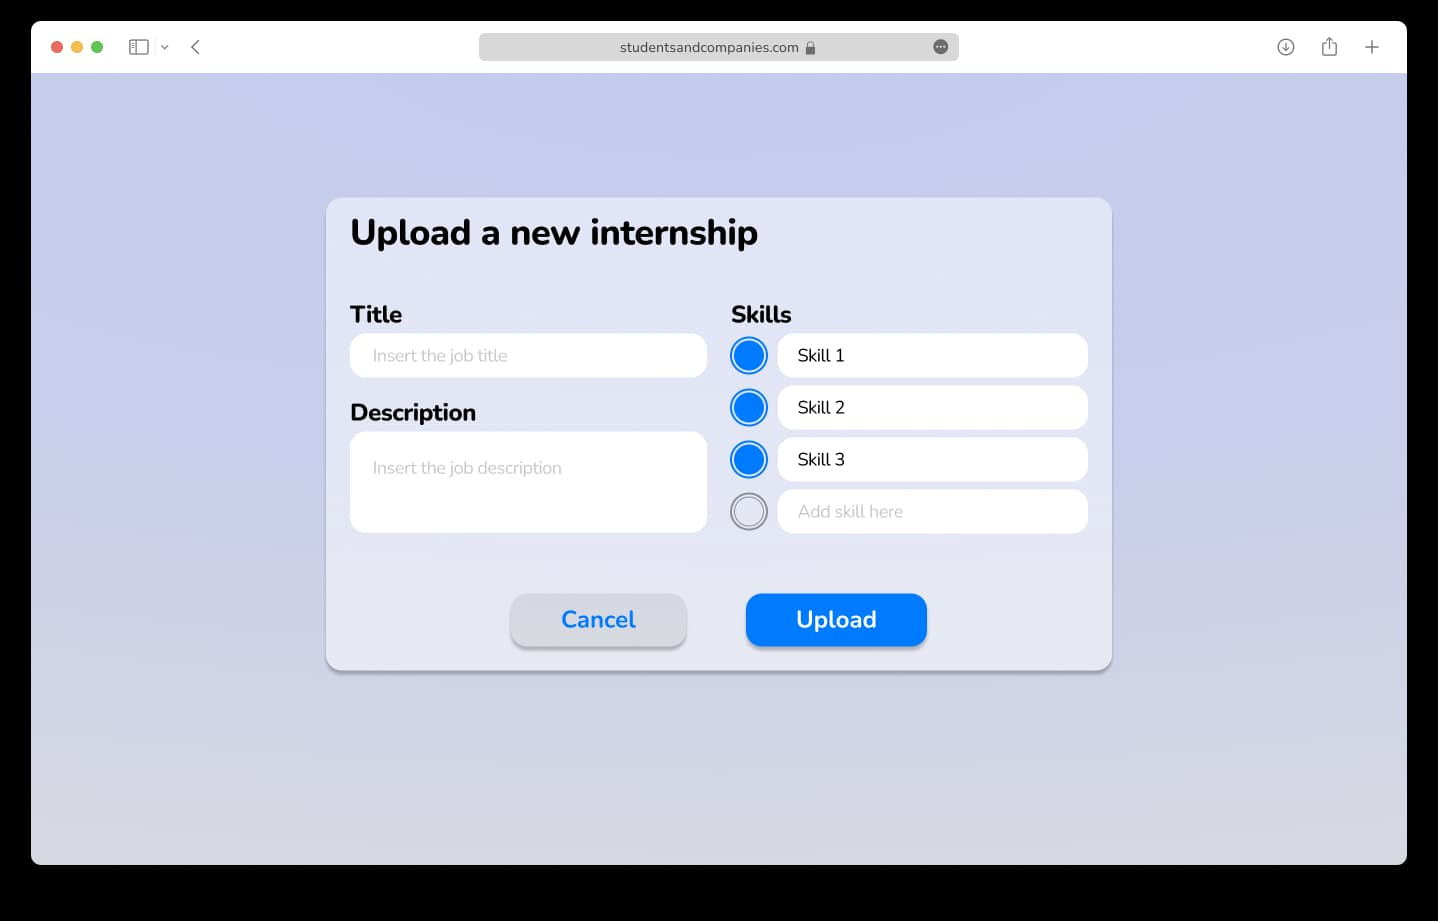
\includegraphics[width=\textwidth]{Images/MockUps/upload_internship.jpeg}\\\\
Monitor Status\\\\
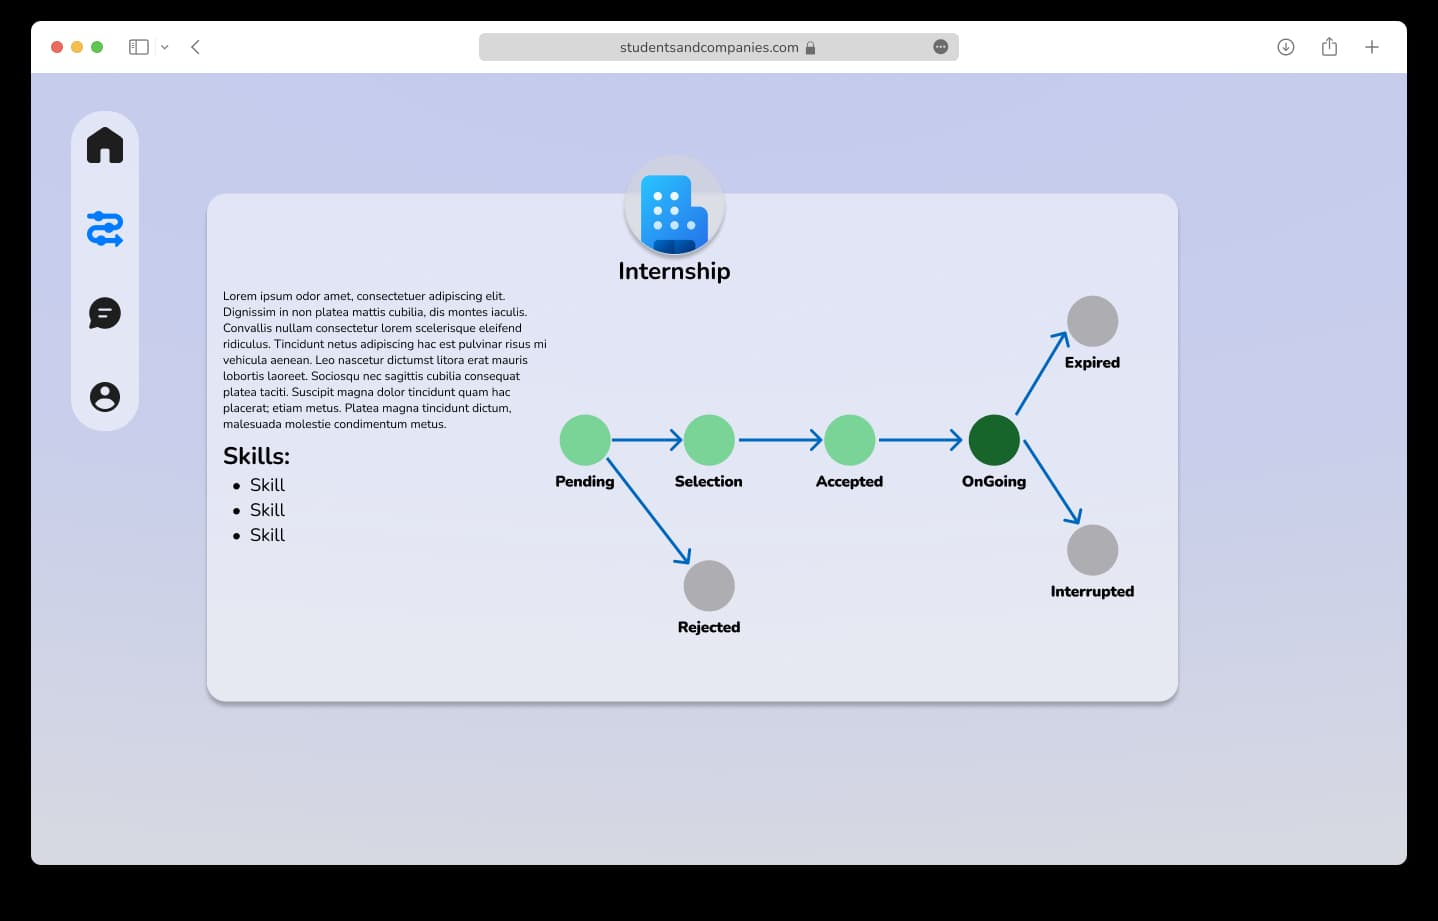
\includegraphics[width=\textwidth]{Images/MockUps/monitor_status.jpeg}

\clearpage
{\color{Blue}{\section{Requirements Traceability}}}
\label{sect:requirements}
\rmtab{
\textbf{Login}\newline
[R1] The system must allow students to log-in through their academic email and password, if they provide them correctly.\newline
[R2] Only students with an academic credential provided by a registered university can log-in.
}{
WebApp \newline
AuthenticationManager\newline
SheerId API\newline
DAO\newline
Database
}

\rmtab{
\textbf{Edit profile}\newline
[R3] The system must allow the student to edit his profile info, remove the CV and add a new version of the CV.\newline
[R4] The student can edit only his profile.
}{
WebApp \newline
AuthenticationManager \newline
AccountManager \newline
DAO \newline
Database
}

\rmtab{
\textbf{Internship recommendation}\newline
[R5] The system must send an email to the student when an internship that might interest him
becomes available.
}{
Affinity Analyzer\newline
DAO\newline
Database\newline
Notification Manager\newline
Mail Service
}

\rmtab{
\textbf{Search an internship}\newline
[R6] The system must provide to the student all internships satisfying search criteria.\newline
[R7] The system must provide to the student only internships satisfying search criteria.
}{
WebApp\newline
Internship Manager\newline
DAO\newline
Database
}
\rmtab{
\textbf{Apply for an internship}\newline
[R8] The system must register the student’s application for the internship.\newline
[R9] The system must register only applications of students who have submitted an application for
the internship.
}{
WebApp\newline
Internship Manager\newline
DAO\newline
Database
}\rmtab{
\textbf{Answer interview questions}\newline
[R10] The student must be able to answer interview questionnaires.\newline
[R11] The student can answer interview questionnaires regarding only internships he’s applied for
and accepted by the involved company.
}{
WebApp\newline
Contract Manager\newline
Interview Manager\newline
DAO\newline
Database
}\rmtab{
\textbf{Consulting CV suggestion}\newline
[R12] The student must be able to view suggestions on how to improve his CV.\newline
[R13] The student can view suggestions regarding only his CV.
}{
CV Analyzer\newline
Notification Manager\newline
Mail Service\newline
DAO\newline
Database
}
\rmtab{
\textbf{Registration and login}\newline
[R14] The system must allow companies to register to S\&C providing mandatory data (name, email,
VAT number) and selecting a password.\newline
[R15] The system must allow registered companies to log-in through their email and password, if they are provided correctly.
}{
WebApp\newline
Authentication Manager\newline
DAO\newline
Database
}\rmtab{
\textbf{Upload an internship}\newline
[R16] The system must allow the company to fill an internship creation form.\newline
[R17] The system must allow the company to select the internship type.\newline
[R18] The system must allow the company to select the internship duration.\newline
[R19] The system must allow the company to select if the internship is paid or not.\newline
[R20] The system must allow the company to select the skills it is searching for in the candidates.
}{
WebApp\newline
Internship Manager\newline
DAO\newline
Database
}
\rmtab{
\textbf{Student recommendation}\newline
[R21] The system must send an email notifying the company when a student with a CV corresponding
to their needs becomes available.
}{
Mail Service\newline
Notification Manager\newline
Affinity Analyzer\newline
DAO\newline
Database
}
\rmtab{
\textbf{Interview students}\newline
[R22] The company must be able to provide structured questionnaires to students.\newline
[R23] The company can provide structured questionnaires only to students who have applied to an internship uploaded by the company itself.\newline
[R24] The company must be able to view answers to questionnaires it created.
}{
WebApp\newline
Contract Manager\newline
Interview Manager\newline
DAO\newline
Database
}
\rmtab{
\textbf{Create contract}\newline
[R25] The company must be able to register a contract regarding an internship and referring to the assigned student.\newline
[R26] The company can register contracts regarding only internships uploaded by the company itself. \newline
[R27] The company can register contracts referring only to students that have applied for the indicated internship.
}{
WebApp\newline
Contract Manager\newline
DAO\newline
Database
}
\rmtab{
\textbf{Login}\newline
[R28] The system must allow registered universities to log-in through credentials provided by S\&C,
if they are provided correctly.
}{
WebApp\newline
Authentication Manager\newline
DAO\newline
Database
}
\rmtab{
\textbf{Terminate an internship}\newline
[R29] The system must allow universities to terminate an internship involving their students.
}{
WebApp\newline
Contract Manager\newline
DAO\newline
Database
}
\rmtab{
\textbf{Leave a feedback}\newline
[R30] The student must be able to post feedback.\newline
[R31] The company must be able to post feedback.\newline
[R32] Only students that have participated in an internship can leave feedback for it.\newline
[R33] Only companies that have participated in an internship can leave feedback for it.\newline
[R34] Every student can leave at most one feedback per internship.\newline
[R35] Every company can leave at most one feedback per internship.\newline
}{
WebApp\newline
Contract Manager\newline
Feedback Manager\newline
DAO\newline
Database
}
\rmtab{
\textbf{Open discussion}\newline
[R36] The student must be able to open a discussion with the company he’s interning with and the
university he’s enrolled at.\newline
[R37] The company must be able to open a discussion with the students they are collaborating with
and universities those students are enrolled at.\newline
[R38] The student can open a discussion only with the company he’s interning with and the university
he’s enrolled at.\newline
[R39] The company can open a discussion only with students they are collaborating with and universities.
}{
WebApp\newline
Contract Manager\newline
Discussion Manager\newline
DAO\newline
Database
}
\rmtab{
\textbf{Send and receive messages within a discussion}\newline
[R40] The student can send and receive messages only from a discussion he is participating in.\newline
[R41] The company can send and receive messages only from a discussion it is participating in.\newline
[R42] The university can send and receive messages only from a discussion it is participating in.
}{
WebApp\newline
Contract Manager\newline
Discussion Manager\newline
DAO\newline
Database
}
\rmtab{
\textbf{Monitor the status of the internship}\newline
[R43] The student must be able to monitor the status of the internships in which he has applied.\newline
[R44] The company must be able to monitor the status of the internships it has published.\newline
[R45] The university must be able to monitor the status of the internship in which its students have applied.
}{
WebApp\newline
Contract Manager\newline
DAO\newline
Database
}

\clearpage
{\color{Blue}{\section{Implementation, Integration, and Test Plan}}}
\label{sect:testing}
\subsection{Overview}
This section goes over how the S\&C platform will be implemented and tested. Through testing it is possible to identify and correct possible bugs proactively, greatly decreasing the risk of a user having problems while using Students\&Companies. In the following sections it will be described how the system will be implemented and how its components will be tested.

\subsection{Testing and Implementation Plan}
The system will be tested and implemented using a bottom-up approach, incrementally adding components as their dependencies are fully tested and integrated. This means that every component will be using its actual dependencies and will be activated by drivers that simulate the behaviour of the upstream components. This testing flow has the advantage of being straightforward and easy to adopt since it reduces the number of mock components that must be created and many components have the same dependencies hence they can be tested simultaneously, speeding up the implementation process.
\\
\begin{figure}[h]
    \centering
    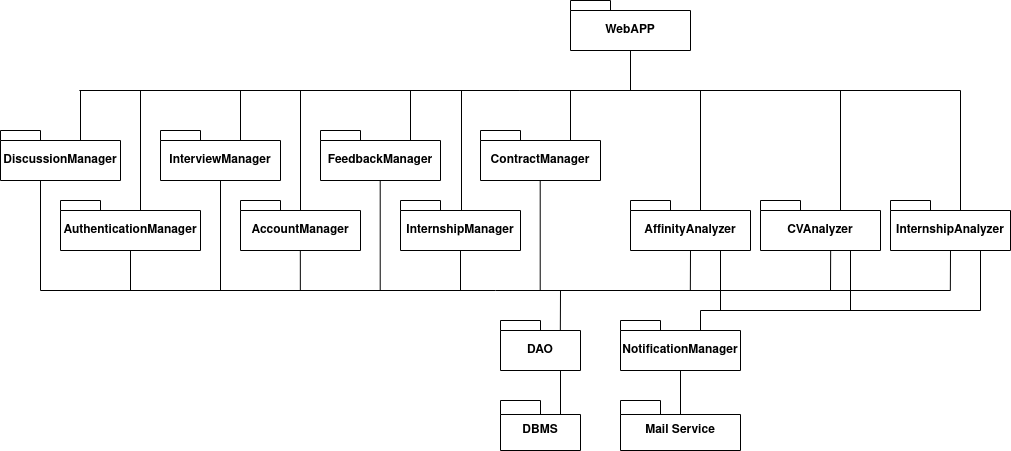
\includegraphics[width=1\linewidth]{Images/testing.drawio(1).png}
    \caption{Dependencies of the components}
    \label{fig:compdep}
\end{figure}
\\
In figure \ref{fig:compdep} are represented by the dependencies between components. Using the bottom-up approach means that for example, the analyzers will be tested after the testing of DAO and NotificationManager is completed. To test the WebAPP component the REST API will be used to submit requests and check that the responses are correct and no errors occur.

\subsection{Additional System Testing}
After the system is fully implemented, there are other aspects which can be tested to ensure that the platform is able to guarantee non-functional requirements such as availability, security and response times. To check this aspects the following tests can be done:
\begin{itemize}
    \item \textbf{Performance testing}: a basic test in which requests are submitted simulating the expected load. This can be used to ensure that everything works as expected under normal conditions, resulting in a positive user experience, and to identify possible bottlenecks or inefficiencies.
    \item \textbf{Stress testing}: there is a possibility of the system receiving more requests than expected. By generating an artificially high number of requests it will be tested if the system is able to handle them or, in the eventuality of crashes due to the high load, is able to gracefully recover.
    \item \textbf{Security testing}: this test is aimed at finding possible vulnerabilities on the platform. This is performed by checking that malicious requests are successfully rejected.
\end{itemize}

\clearpage
\color{Blue}{\section{Effort Spent}}
\label{sect:effort}
\textcolor{Black}{
\\
Bogdanovic Stefan\\
\begin{tabular}[h]{|c|c|}
    \hline
    Section & Effort spent \\
    \hline
    1 & 1 \\
    \hline
    2 & 14 \\
    \hline
    3 & 2 \\
    \hline
    4 & 8 \\
    \hline
    5 & 1 \\
    \hline
\end{tabular}
\\ \\
Rodari Simone\\
\begin{tabular}[h]{|c|c|}
    \hline
    Section & Effort spent \\
    \hline
    1 & 1 \\
    \hline
    2 & 16 \\
    \hline
    3 & 8 \\
    \hline
    4 & 2 \\
    \hline
    5 & 1 \\
    \hline
\end{tabular}
\\ \\
Pignataro Gabriele\\
\begin{tabular}[h]{|c|c|}
    \hline
    Section & Effort spent \\
    \hline
    1 & 1 \\
    \hline
    2 & 12 \\
    \hline
    3 & 2 \\
    \hline
    4 & 3 \\
    \hline
    5 & 6 \\
    \hline
\end{tabular}
}

\clearpage
\addcontentsline{toc}{section}{References}
\bibliographystyle{plain}
\bibliography{main}

\end{document}